% !TeX root = ./main.tex
% !TEX TS-program = xelatex

\documentclass[russian,utf8,simple]{eskdtext}

\usepackage{cmap}
\usepackage{fontspec}
\usepackage{xecyr}
\usepackage{graphicx}
\usepackage{amsmath}
\usepackage{titlesec}
\usepackage{tocloft}
\usepackage{eqexpl}
\usepackage{ltxtable}
\usepackage{icomma}
\usepackage{indentfirst}
\usepackage{enumitem}
\usepackage{caption}
\usepackage{float}
\usepackage{tikz}
\usepackage{pdfpages}
\usepackage{fancyvrb}

\def\checkmark{\tikz\fill[scale=0.4](0,.35) -- (.25,0) -- (1,.7) -- (.25,.15) -- cycle;} 
\def\centersection#1{\hspace{6cm} #1}

\eqexplSetDelim{~--}
\eqexplSetIntro{где}

\sloppy

\setcounter{tocdepth}{2}
\setcounter{secnumdepth}{4}

\setlength{\cftsubsecindent}{0cm}
\setlength{\cftbeforesecskip}{0pt}
\setlength\parindent{5ex}

\setlist[enumerate,1]{label=\arabic*)}
\setlist[enumerate,2]{label=\arabic*),leftmargin=1.5cm}

\setlist{nolistsep,parsep=0pt,leftmargin=1.6cm,wide}

\setlist[2]{labelindent=2\parindent,leftmargin=1.3cm}

\newcommand{\No}{\textnumero}

% Thank: https://stackoverflow.com/questions/2785260/hide-an-entry-from-toc-in-latex
\newcommand{\nocontentsline}[3]{}
\newcommand{\tocless}[2]{\bgroup\let\addcontentsline=\nocontentsline#1{#2}\egroup}

\renewcommand{\ESKDcolumnXfIname}{Студент}
\renewcommand{\ESKDcolumnXfIIname}{Консульт.}
\renewcommand{\ESKDcolumnXfVname}{Руковод.}
\renewcommand{\ESKDcolumnXfVIname}{Н. контр.}

\renewcommand{\arraystretch}{1.3}

\renewcommand{\cfttoctitlefont}{\hfill\normalfont}
\renewcommand{\cftaftertoctitle}{\hfill\hfill}

\renewcommand{\cftsecfont}{\normalfont}
\renewcommand{\cftsecpagefont}{\normalfont}

\renewcommand{\cftsecleader}{\cftdotfill{\cftdotsep}}

% Меня это жутко раздражает. Из-за "ГОСТ"а моей шараги мой дип. рук стал норм.контролером.
% Ох.еть

\ESKDtitle{\textnormal{{\footnotesize Разработка серверной части для онлайн-конструктора конфигураций}}}
\ESKDsignature{\textnormal{РКСИ.ВКР20.09.02.03.2297.00ПЗ}}
\ESKDauthor{Леммер}
\ESKDnormContr{Ляхов}
\ESKDchecker{Езепчук}
\ESKDapprovedBy{Жабинская}

\graphicspath{{img/}}

\setmainfont[Mapping=tex-text]{Times New Roman}
\setsansfont[Mapping=tex-text]{Liberation Sans}
\setmonofont[Mapping=tex-text]{Liberation Mono}

\titleformat{\section}{\normalfont\normalsize}{\thesection}{1em}{}
\titleformat{\subsection}{\normalfont\normalsize}{\thesubsection}{1em}{}
\titleformat{\subsubsection}{\normalfont\normalsize}{\thesubsubsection}{1em}{}
\titleformat{\paragraph}
{\normalfont\normalsize}{\theparagraph}{1em}{}
\titlespacing*{\paragraph}
{5ex}{1.5cm}{1.5cm}

\linespread{1}

\captionsetup[figure]{skip=0.5cm}

\captionsetup[table]{format=hang,indention=-60pt,margin=5ex}

\begin{document}
    \ESKDthisStyle{empty}
\begin{center}
\textbf{{\footnotesize
    МИНИСТЕРСТВО ОБЩЕГО И ПРОФЕССИОНАЛЬНОГО ОБРАЗОВАНИЯ\\РОСТОВСКОЙ ОБЛАСТИ\\
    ГОСУДАРСТВЕННОЕ БЮДЖЕТНОЕ ПРОФЕССИОНАЛЬНОЕ ОБРАЗОВАТЕЛЬНОЕ
    УЧРЕЖДЕНИЕ РОСТОВСКОЙ
    ОБЛАСТИ\\РОСТОВСКИЙ-НА-ДОНУ КОЛЛЕДЖ СВЯЗИ И ИНФОРМАТИКИ
    }
}
\end{center}
\vfill
    \hspace{11.5cm} ДОПУСТИТЬ К ЗАЩИТЕ

    \noindent \hspace{10cm} Председатель цикловой комиссии

    \noindent \hspace{12.5cm} "<Программирование">

    \noindent \hspace{9.5cm} \rule{4cm}{0.25pt} / E.M. Кротенко /

    \noindent \hspace{11.2cm} "<\rule{1cm}{0.25pt}"> \rule{3cm}{0.25pt} 2020 г.
\vfill
\begin{center}
    \textbf{{\huge
        Выпускная квалификационная\\ работа
    }}
\end{center}
\vfill
\textbf{Тема}: \underline{Разработка серверной части
для онлайн конструктора конфигураций}
\vfill
\begin{center}
    ПОЯСНИТЕЛЬНАЯ ЗАПИСКА\\
    $\underset{\text{(шифр)}}{\underline{\text{РКСИ.ВКР20.09.02.03.2297.00ПЗ}}}$
\end{center}
\vfill
Специальность: \underline{Программирование в компьютерных системах}
\vfill
\noindent Нормконтроллер \hspace{2cm} $\underset{\text{(подпись)}}{\rule{3.5cm}{0.25pt}}$ \hspace{0.5cm} Жабинская И.Н.
\vfill
\noindent Руководитель   \hspace{2.7cm} $\underset{\text{(подпись)}}{\rule{3.5cm}{0.25pt}}$ \hspace{0.5cm} Ляхов Н.Е.
\vfill
\noindent Консультант по\\экономической части \hspace{1.10cm} $\underset{\text{(подпись)}}{\rule{3.5cm}{0.25pt}}$ \hspace{0.5cm} Езепчук А.В.
\vfill
\noindent Студент \hspace{4.05cm} $\underset{\text{(подпись)}}{\rule{3.5cm}{0.25pt}}$ \hspace{0.5cm} Леммер Э.С. \hspace{0.3cm} Группа \underline{ПОКС-42}

\begin{center}{\footnotesize
    2020 г.
}
\end{center}
    \newpage
    \ESKDthisStyle{formII}
\tocloftpagestyle{empty}
\tableofcontents
    \newpage
    \section*{\centersection{Введение}}
\addcontentsline{toc}{section}{Введение}

В разработке больших программных продуктов, а в
особенности тех, что используют сервисно-подобную
архитектуру, сегодня всё чаще используется система контейнеризации Docker.

Docker – это программная платформа для быстрой разработки, тестирования
и развертывания приложений как на промышленном сервере, так и на устройстве
каждого разработчика. Docker упаковывает ПО в стандартизованные блоки,
которые называются контейнерами. Каждый контейнер включает все необходимое для
работы приложения: библиотеки, системные инструменты, код и среду исполнения.
Благодаря Docker можно быстро развертывать и масштабировать приложения в любой
среде и сохранять уверенность в том, что код будет работать.

В приложениях, основанных на микросервисной архитектуре, то есть архитектуре программного
обеспечения, ориентированной на взаимодействие насколько это возможно небольших,
слабо связанных и легко изменяемых модулей, очень важно установить правила взаимодействия
микросервисов между собой. В случае с контейнеризацией при помощи Docker, для этого
существует система docker-compose, которая использует файл docker-compose.yaml, в котором
описаны все настройки приложения, основанного на независимых модулях.

Написание данного файла вручную часто связано с неудобствами и возможностью ошибиться
и, тем самым подвергнуть всю инфраструктуру проекта различным рискам.

В рамках подготовки к написанию выпускной квалификационной работы была озвучена
идея создания онлайн сервиса, способного облегчить, структурировать и автоматизировать
работу над написанием docker-compose.yaml и минимизировать вероятность получения неудворительного
результата из-за невнимательности или неопытности разработчика, а также иных обстоятельств.

Дополнительно, пользователю можно будет предоставить возможность хранить множество
конфигураций под разные проекты, делиться ими с членами команды, а также использовать
наработки других разработчиков для облегчения своей задачи и развития технологии контейнеризации.

Для приложения данного типа идеально подходит платформа web, так как этом случае пользователю не требуется:


\begin{itemize}
    \item xранить тяжеловесное ПО у себя на машине, так как основная часть находится на сервере;
    \item не понадобится устанавливать обновления;
    \item cервисом можно будет пользоваться с любого устройства, работающего под любой операционной системой.
\end{itemize}

Более того, web-приложения легко разворачивать и распространять, минуя различные платформы,
распространяющие мобильные или desktop-приложений и их требования к программным продуктам.

Идея была воплощена в онлайн сервисе “Сonfig Castle” - сайте, предоставляющем все вышеперечисленные функции в полном объёме.

В дальнейшем речь пойдет о всех этапах проектирования и тестирования данного сервиса.


    \newpage
    \section{Сбор и анализ требований}

\vspace{-0.9cm}

\subsection{Этап сбора требований}

\label{req:sect_1}

Подэтапы сбора требований включают в себя:

\begin{itemize}[wide]
    \item анкетирование целевой аудитории;
    \item тзучение рынка на предемет конкурентов;
    \item мозговой штурм.
\end{itemize}

\subsubsection{Анкетирование целевой аудитории}

В рамках сбора требований к программному продукту было проведено анкетирование целевой аудитории проекта. В состав анкеты вошли следующие вопросы:

\begin{enumerate}
    \item "<Кто вы в IT?">;
    \item "<Часто ли вы имеете дело с файлом docker-compose.yaml?">;
    \item "<Используете ли вы специальные средства для редактирования docker-compose.yaml?">;
    \item "<Хотели бы вы иметь под рукой графический интерфейс со множеством возможностей для редактирования docker-compose.yaml?">;
    \item "<Пожалуйста, опишите желаемые возможности подобного инструмента.">.
\end{enumerate}

Диаграмма ответов на первый вопрос приведён на рисунке \ref{req:first_q}.

\begin{figure}[H]
        \center{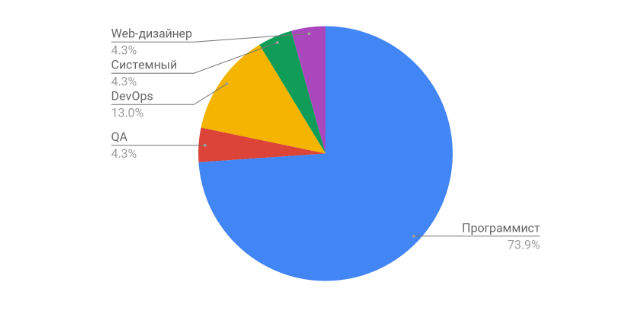
\includegraphics[scale=0.7]{first_q.png}}
        \caption{Ответы на первый вопрос анкеты}
        \label{req:first_q}
\end{figure}

Ответы на первый вопрос поможет уточнить уточнить состав целевой аудитории по направлениям в IT.

Исходя из результатов, отображённых на рисунке \ref{req:first_q} можно сделать следующие выводы:
\begin{itemize}
    \item не потребуется поддержка старых браузеров, так как программисты технически заточены и шанс, что кто-то из них будет использовать Internet Explorer ниже 11 версии низок;
    \item цветовая палитра рабочей области должна быть в тёмных тонах, так как большинство программистов используют в IDE и текстовых редакторов тёмную тему оформления.
\end{itemize}

Диаграмма результатов ответа на второй вопрос привидена на рисунке \ref{req:second_q}.

\begin{figure}[H]
    \center{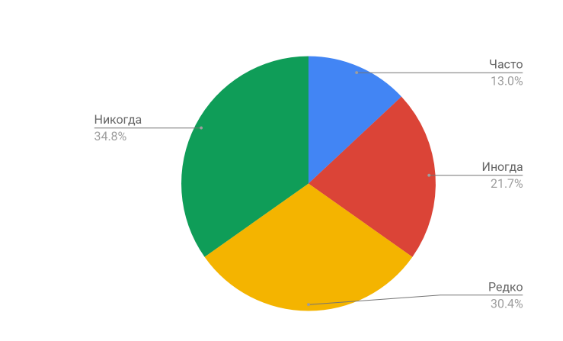
\includegraphics[scale=0.7]{second_q.png}}
    \caption{Ответы на второй вопрос анкеты}
    \label{req:second_q}
\end{figure}

Ответы помогут нам понять, как часто будет пригождаться тем или иным пользователям наш продукт. Делая вывод, можно понять, что
требуется сделать акцент на том, что значительная часть пользователей сервиса будут использовать его не единожды. Это значит, что нужно дать пользователю возможность получать доступ к ранее созданным файлам конфигураций в рамках сервиса. За это должна взиматься плата в виде ежемесячной подписки.

Ответы на третий вопрос позволяют узнать ранее незамечанных конкурентов при разработке идеи проекта. Абсолютно все участники опроса ответили на него отрицательно.

Диаграмма ответов опрашиваемых на четвёртый вопрос привидена на рисунке \ref{req:fourth_q}.

\begin{figure}[H]
    \center{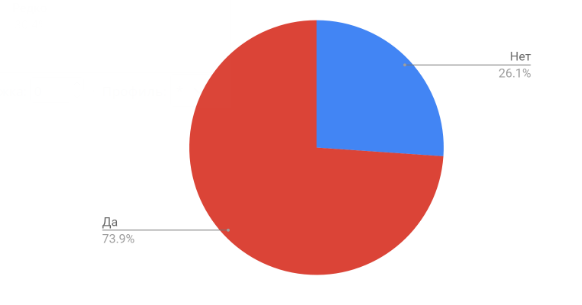
\includegraphics[scale=0.7]{fourth_q.png}}
    \caption{Ответы на четвёртый вопрос анкеты}
    \label{req:fourth_q}
\end{figure}

Ответы на четвёртый вопрос являются главными для проекта, иными словами нужен ли рынку разрабатываемый программный продукт.

Ответов на четвёртый вопрос, к сожалению не поступило.

\subsubsection{Изучение рынка}

В процессе поиска конкурирующего программного обеспечения не было обнаружено серьёзных соперников в данной области. Исключение составляют лишь инструменты, являющиеся обособленными частями рассматриваемого проекта, как то:

\begin{itemize}[wide]
    \item Инструменты для проверки синтаксиса;
    \item Текстовые редакторы;
    \item Различные документации.
\end{itemize}

Также об отсутствии конкурентов на рынке свидетельствуют и результаты анкетирование, приведённые в пункте 1.1.1.

\subsubsection{Мозговой штурм}

По результатам данного этапа сбора требований были выдвинуты следующие идеи:

\begin{itemize}
    \item должно сущестовать две роли пользователей: посетитель и клиент;
    \item в качестве встроенного текстового редактора нужно использовать Monaco Editor - редактор с открытым исходным кодом и большим количеством возможностей в настройке, который можно встраивать на сайт;
    \item приложение не будет активно использоваться на мобильных устройствах, а из этого следует:
    \begin{itemize}
        \item достаточно поддержки десктопных браузеров;
        \item адаптивность страниц под мобильные устройства не требуется.
    \end{itemize}
    \item необходимо наличие сервера, который бы предоставлял данные с базы данных;
    \item необходимо наличие авторизационного сервера, предоставляющего функционал связанные с аутенфикацией и авторизацией.
\end{itemize}

\subsection{Этап анализа и формирования требований}

\label{req:sect_2}

Исходя из темы дипломной работы, необходимо обозначить требования к серверной части проекта исходя из раздела \ref{req:sect_1} для наилучшей работы клиентской части проекта.

Перед утверждением окончательных функциональных требований к разрабатываемому программному продукту, было проведено небольшое исследование с целью получения
лучших способов достичь желаемого, опираясь на уже существующие архитектурные решения серверных приложений.

Дополнительно была проведена беседа с разработчиком клиентской части проекта, где утвердились формат запрашиваемых данных и способо их получения.

Так, данные должны быть полученными в виде json документа, при этом какая информация поступить, в каком порядке должно определяться фронтендм-приложением, а не бекендом.
Вполне резонно в таком случае иметь лишь один uri для обмена данными. Решением данной проблемы служит GraphQL и вся его инфрастуктура. Данное положение выражено только при работе
с окном конфигураций, а сервер авторизации должно работать на архитектуре REST, т.е. иметь множество uri или endpoint-ов, где каждый используется по назначению.

Исходя из вышеобозначенной информаци, можно сформировать общие требования, список которых привидён ниже:
\begin{itemize}
    \item серверная часть сущесвует в виде отдельного и независимого приложения, которое описывает структуру и подход к управлению базой данных, т.е. любой клиент должен иметь возможнось использовать серверное приложение, иными словами бекенд должен выступать как некая спецификая для каждого клиента;
    \item хранение данных должно быть организовано в отдельной базе данных, исходя из принципе сетевого приложения;
    \item сервер работает асинхронно, т.е. не блокирует операции ввода-вывода;
    \item необходимо наличие общего для фротенда API(Application Programming Interface), который сможет производить операции по добавлению, изменению, удалению и чтению данных;
    \item API должен быть реализован с использованием языка запросов GraphQL для масштабируемого и стабильного API;
    \item GraphQL API должен предоставлять такие запросы как file, files, service и services;
    \item GraphQL API должен предоставлять такие мутации как createFile, updateFile и deleteFile;
    \item исходя из принципа доступности сетевых приложений, бекенд должен быть размещён на отдельном веб-сервере для доступности в любое время и работать максимально эффективно без суточных норм;
    \item приложение авторизации и редактора должны существовать отдельно друг от друга и не подозревать о наличии другого;
    \item прилжение интегрируется с Яндекс.Кассой для возможности оплаты регистрации;
    \item существование отдельных ролей: пользователя и клиента.
\end{itemize}

    \newpage
    \section{Проектирование и разработка архитектуры программного продукта}

После анализа требований к разрабатываемому продукту нужно составить все необходимые диаграммы, включая MindMap и UseCase.

\subsection{Построение диаграммы связей}

Для общей наглядности внутренностей проекта была составлена карта связей, она же MindMap, показанная на
рисунке \ref{des:mind_map}.

\begin{figure}[H]
    \center{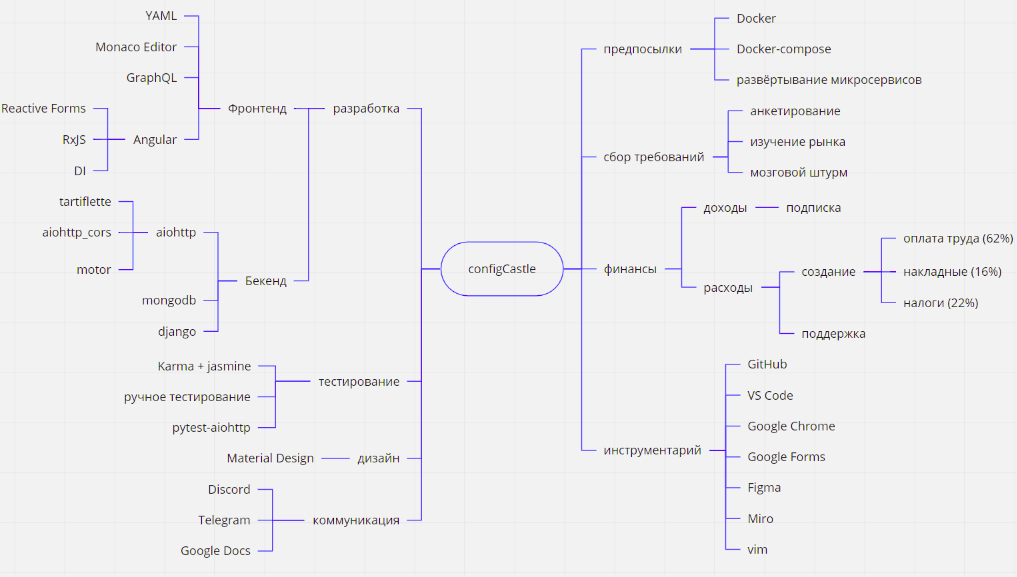
\includegraphics[scale=0.65]{mindmap.png}}
    \caption{Диаграмма связей}
    \label{des:mind_map}
\end{figure}

Здесь показана общая концепция продукта, что стало его предпосылкой, какие инструментальные средства использовались
и так далее.

В дальнейшем можно использовать эту карту, разместив её в wiki проекта для того, чтобы новые разработчики смогли ознакомиться с ней
и приступить к работе с минимальными затратами, понять какую проблему решает продукт, что используется для разработки, как происходит
коммуникация между разработчиками и с какими библиотеками необходимо быть знакомым.

\subsection{Разработка сценария использования}

После анализа ответов на вопрос можно прийти к определённым сценариям взаимодействия с пользователем. Исходя из принципа доступности и легко-понятного
пользовательского интерфейса, можно сконструировать определённые сценарии взаимодействия пользователей с программным продуктом. Результат подобной работы
изображен на так называемой диаграмме UseCase, привидённой на рисунке \ref{des:use_case}.

\begin{figure}[H]
    \center{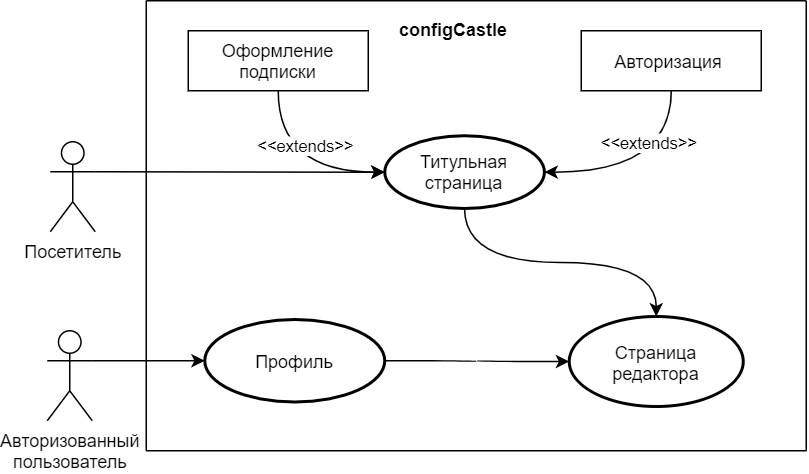
\includegraphics[scale=0.5]{usecase.png}}
    \caption{Диаграмма UseCase}
    \label{des:use_case}
\end{figure}

\subsection{Прототипирование и дизайн программного продукта}

На рисунках \ref{des:proto_1}, \ref{des:proto_2}, \ref{des:proto_3}, \ref{des:proto_4}, \ref{des:proto_5} и
\ref{des:proto_6} показаны прототипы, которые были созданы специально для проекта. Отображены и обозначены основные блоки дизайна, а также различия между
одними и теми же страницами, но с отличаюмещеся ролями пользователей. Так, например, пользователь с подпиской, т.е. клиент имеет функцию сохранить конфигурационный файл
в базе данных и использовать его в дальнейшем тогда как пользователь с ролью посетитель может только создать один файл в реальном времени, не имея возможности обозначенной ранее.

\begin{figure}[H]
    \center{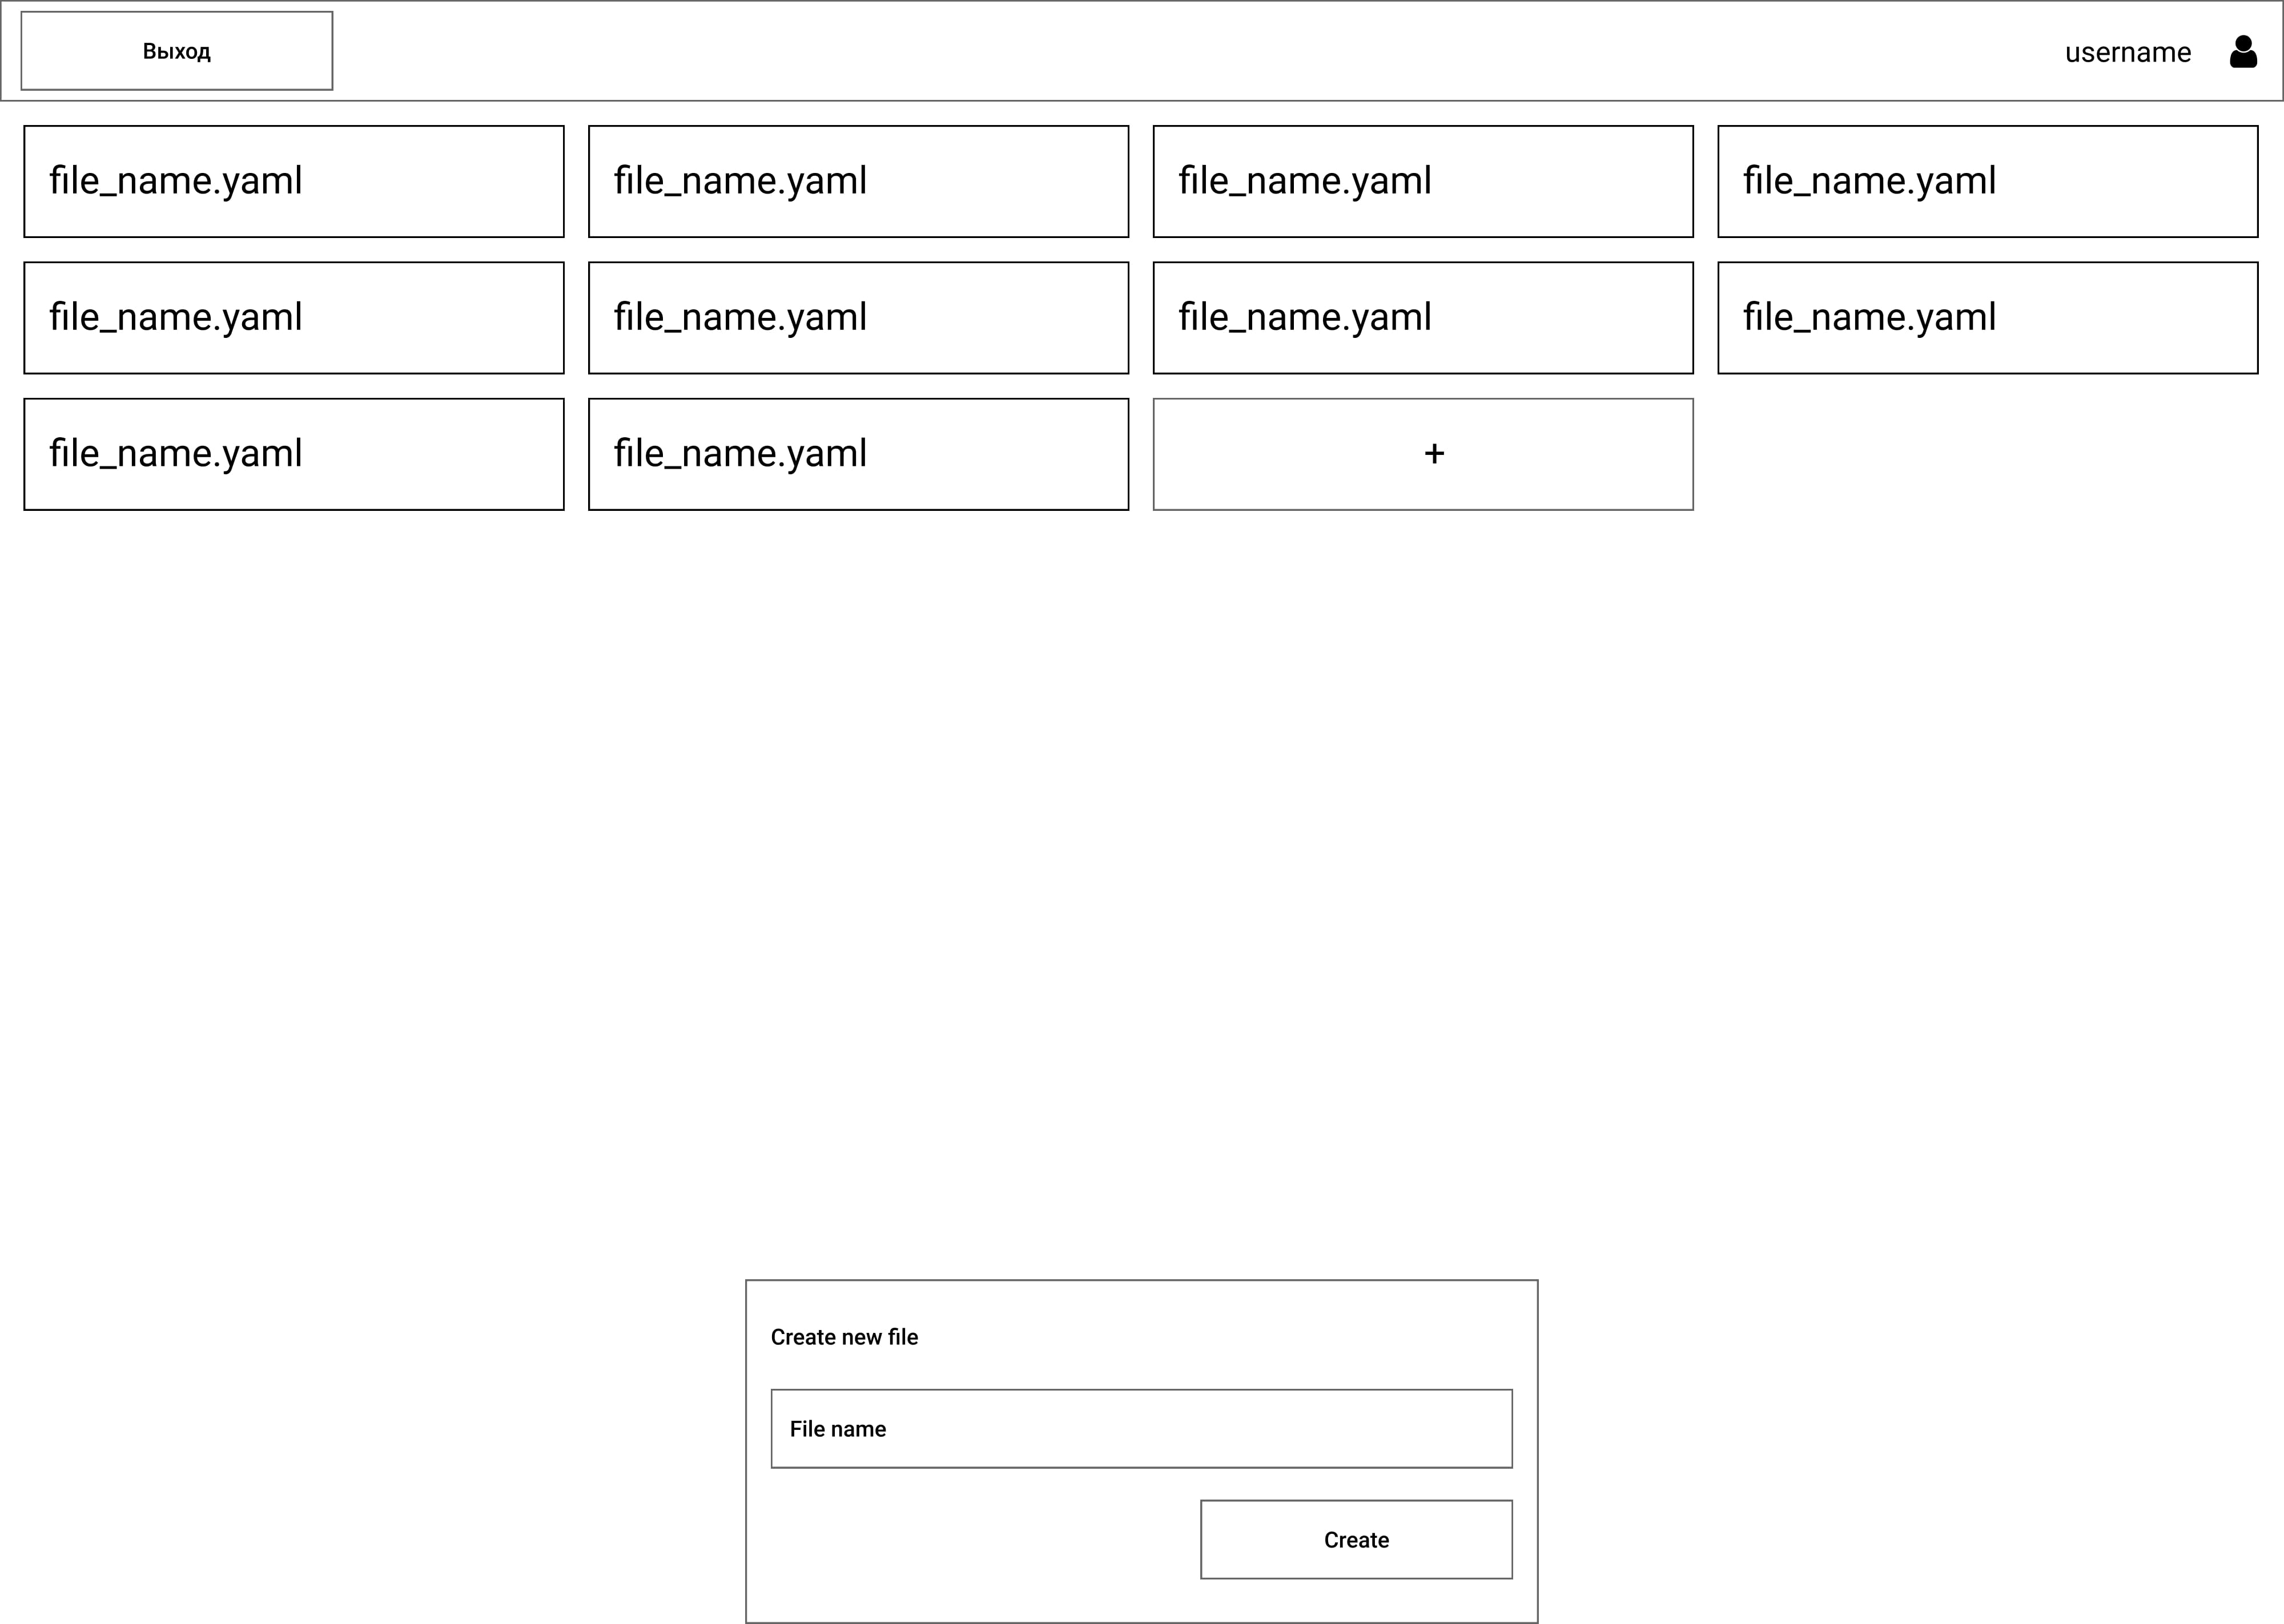
\includegraphics[scale=0.09]{Dashboard.jpg}}
    \caption{Прототип Dashboard-а сайта}
    \label{des:proto_1}
\end{figure}

\begin{figure}[H]
    \center{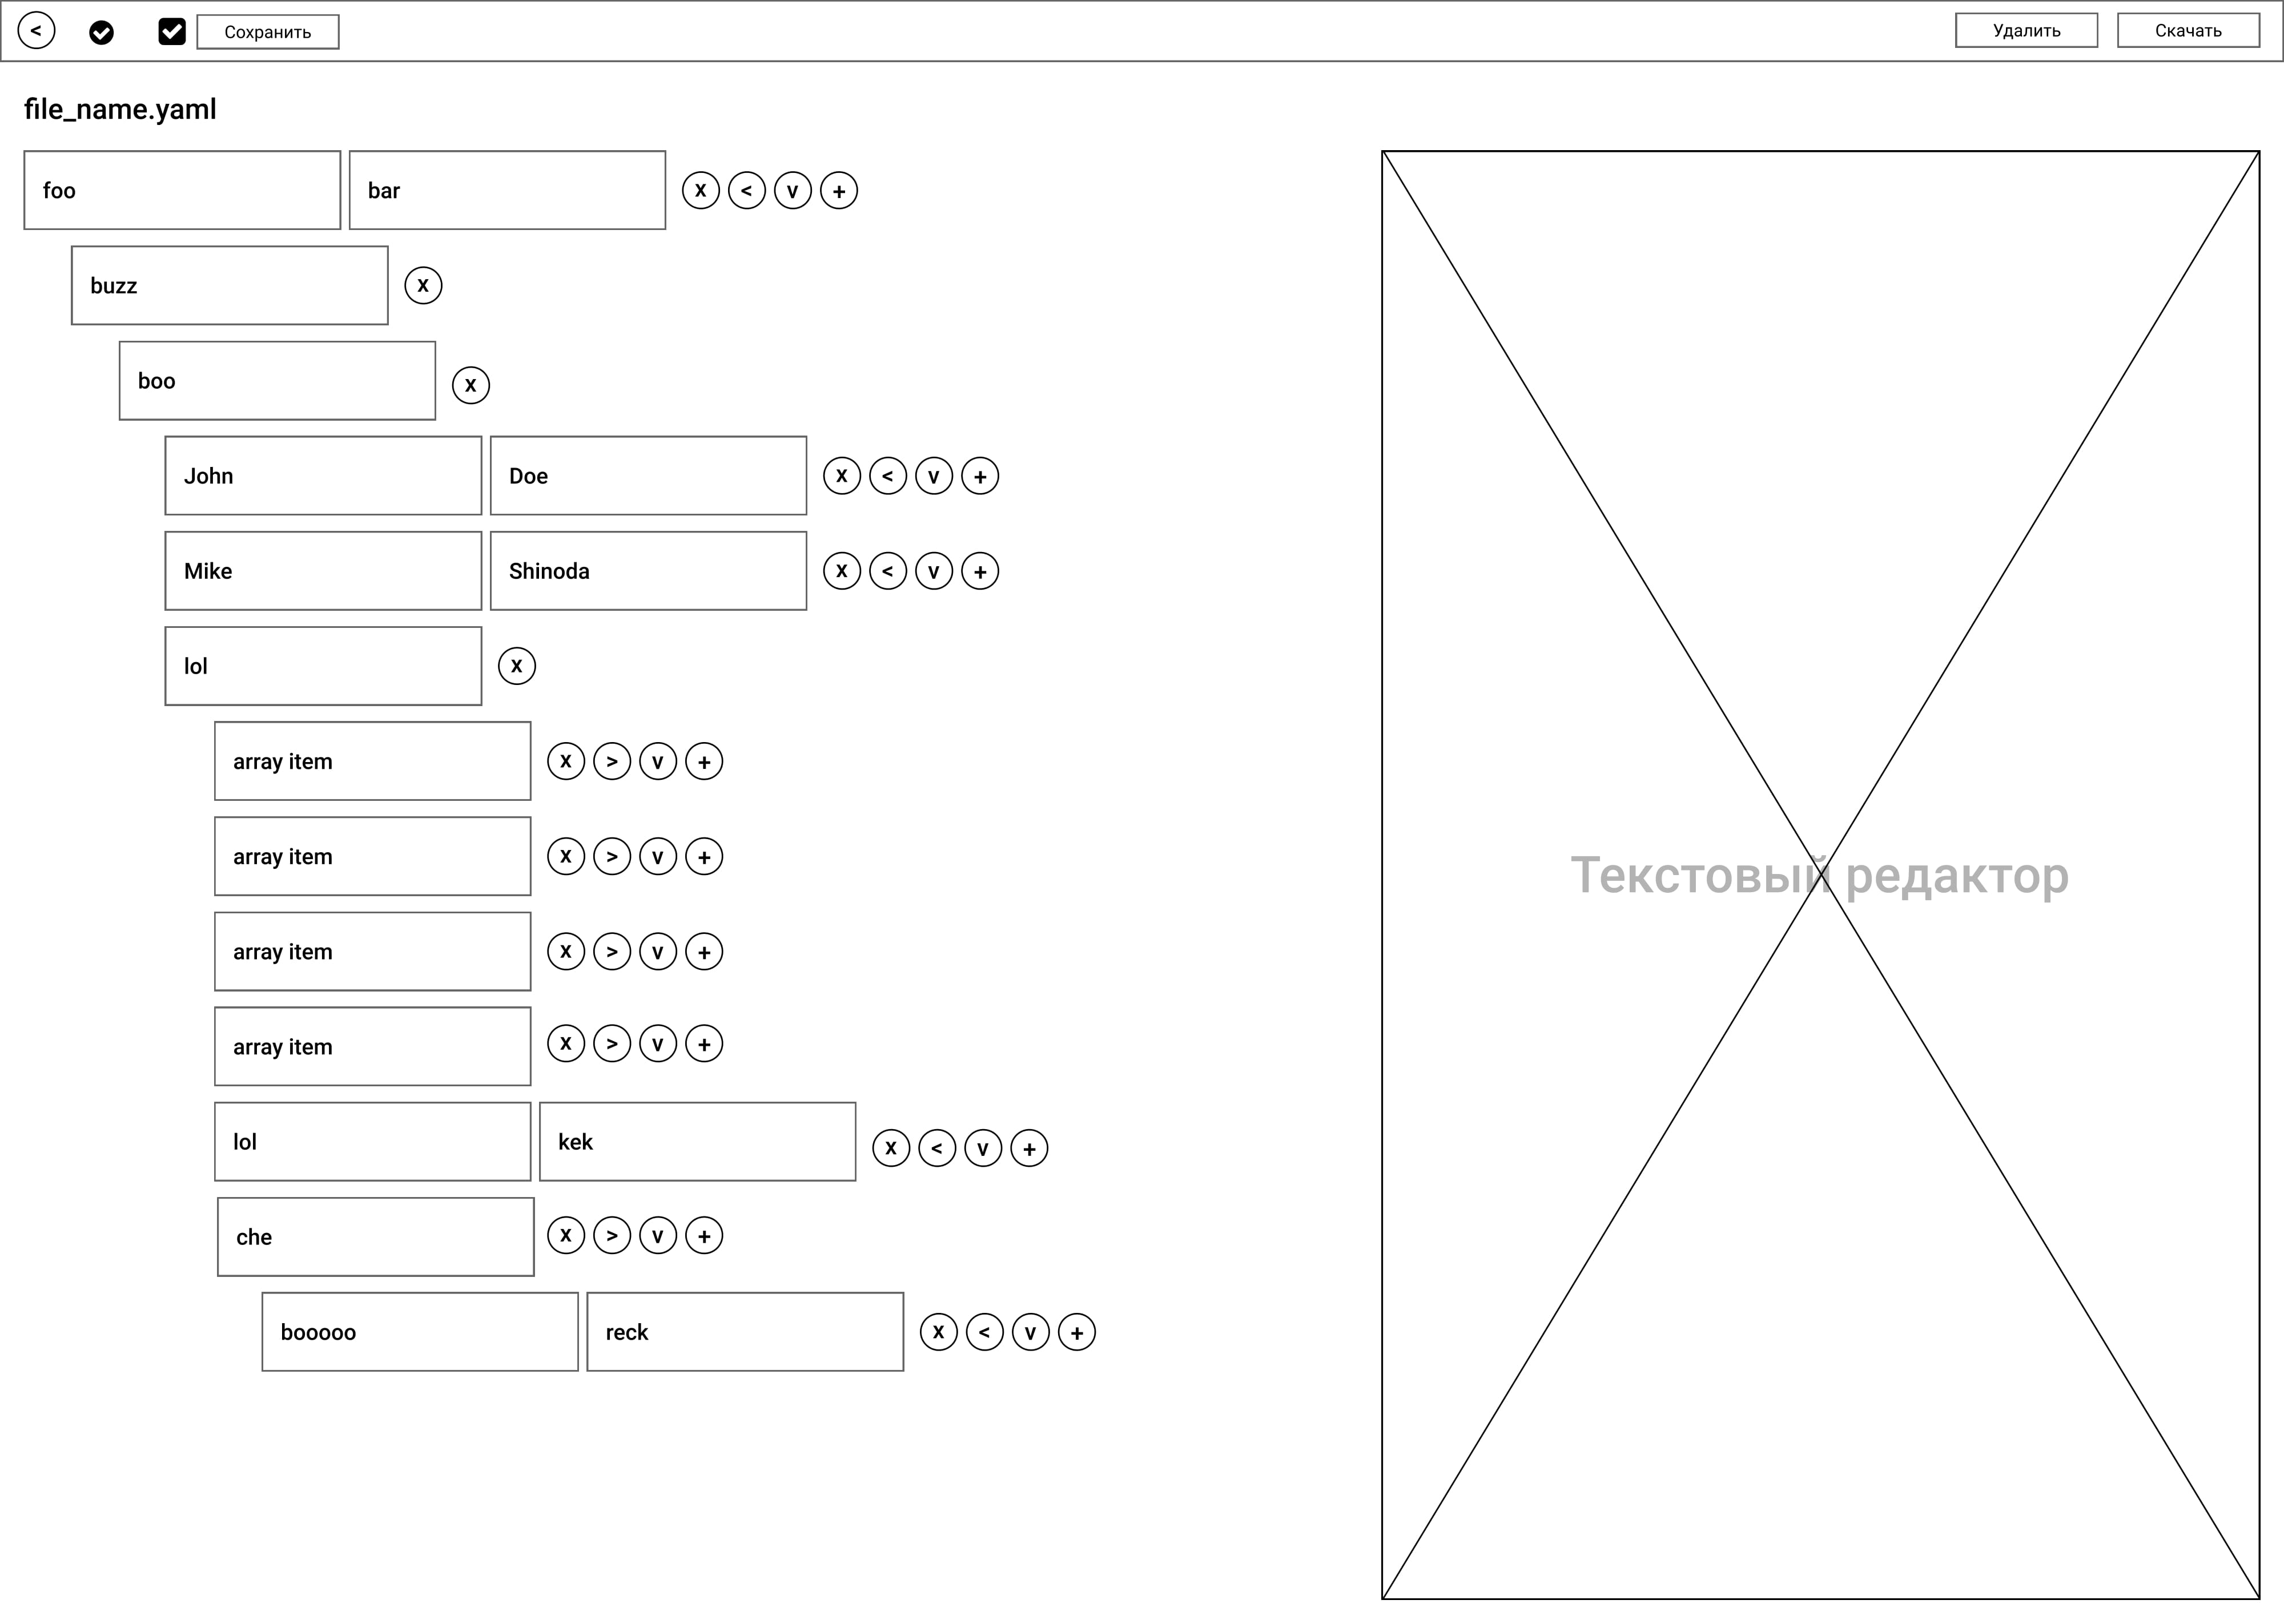
\includegraphics[scale=0.09]{Editor (client).jpg}}
    \caption{Прототип дизайна редактора, если пользователь имеет статус клиента}
    \label{des:proto_2}
\end{figure}

\begin{figure}[H]
    \center{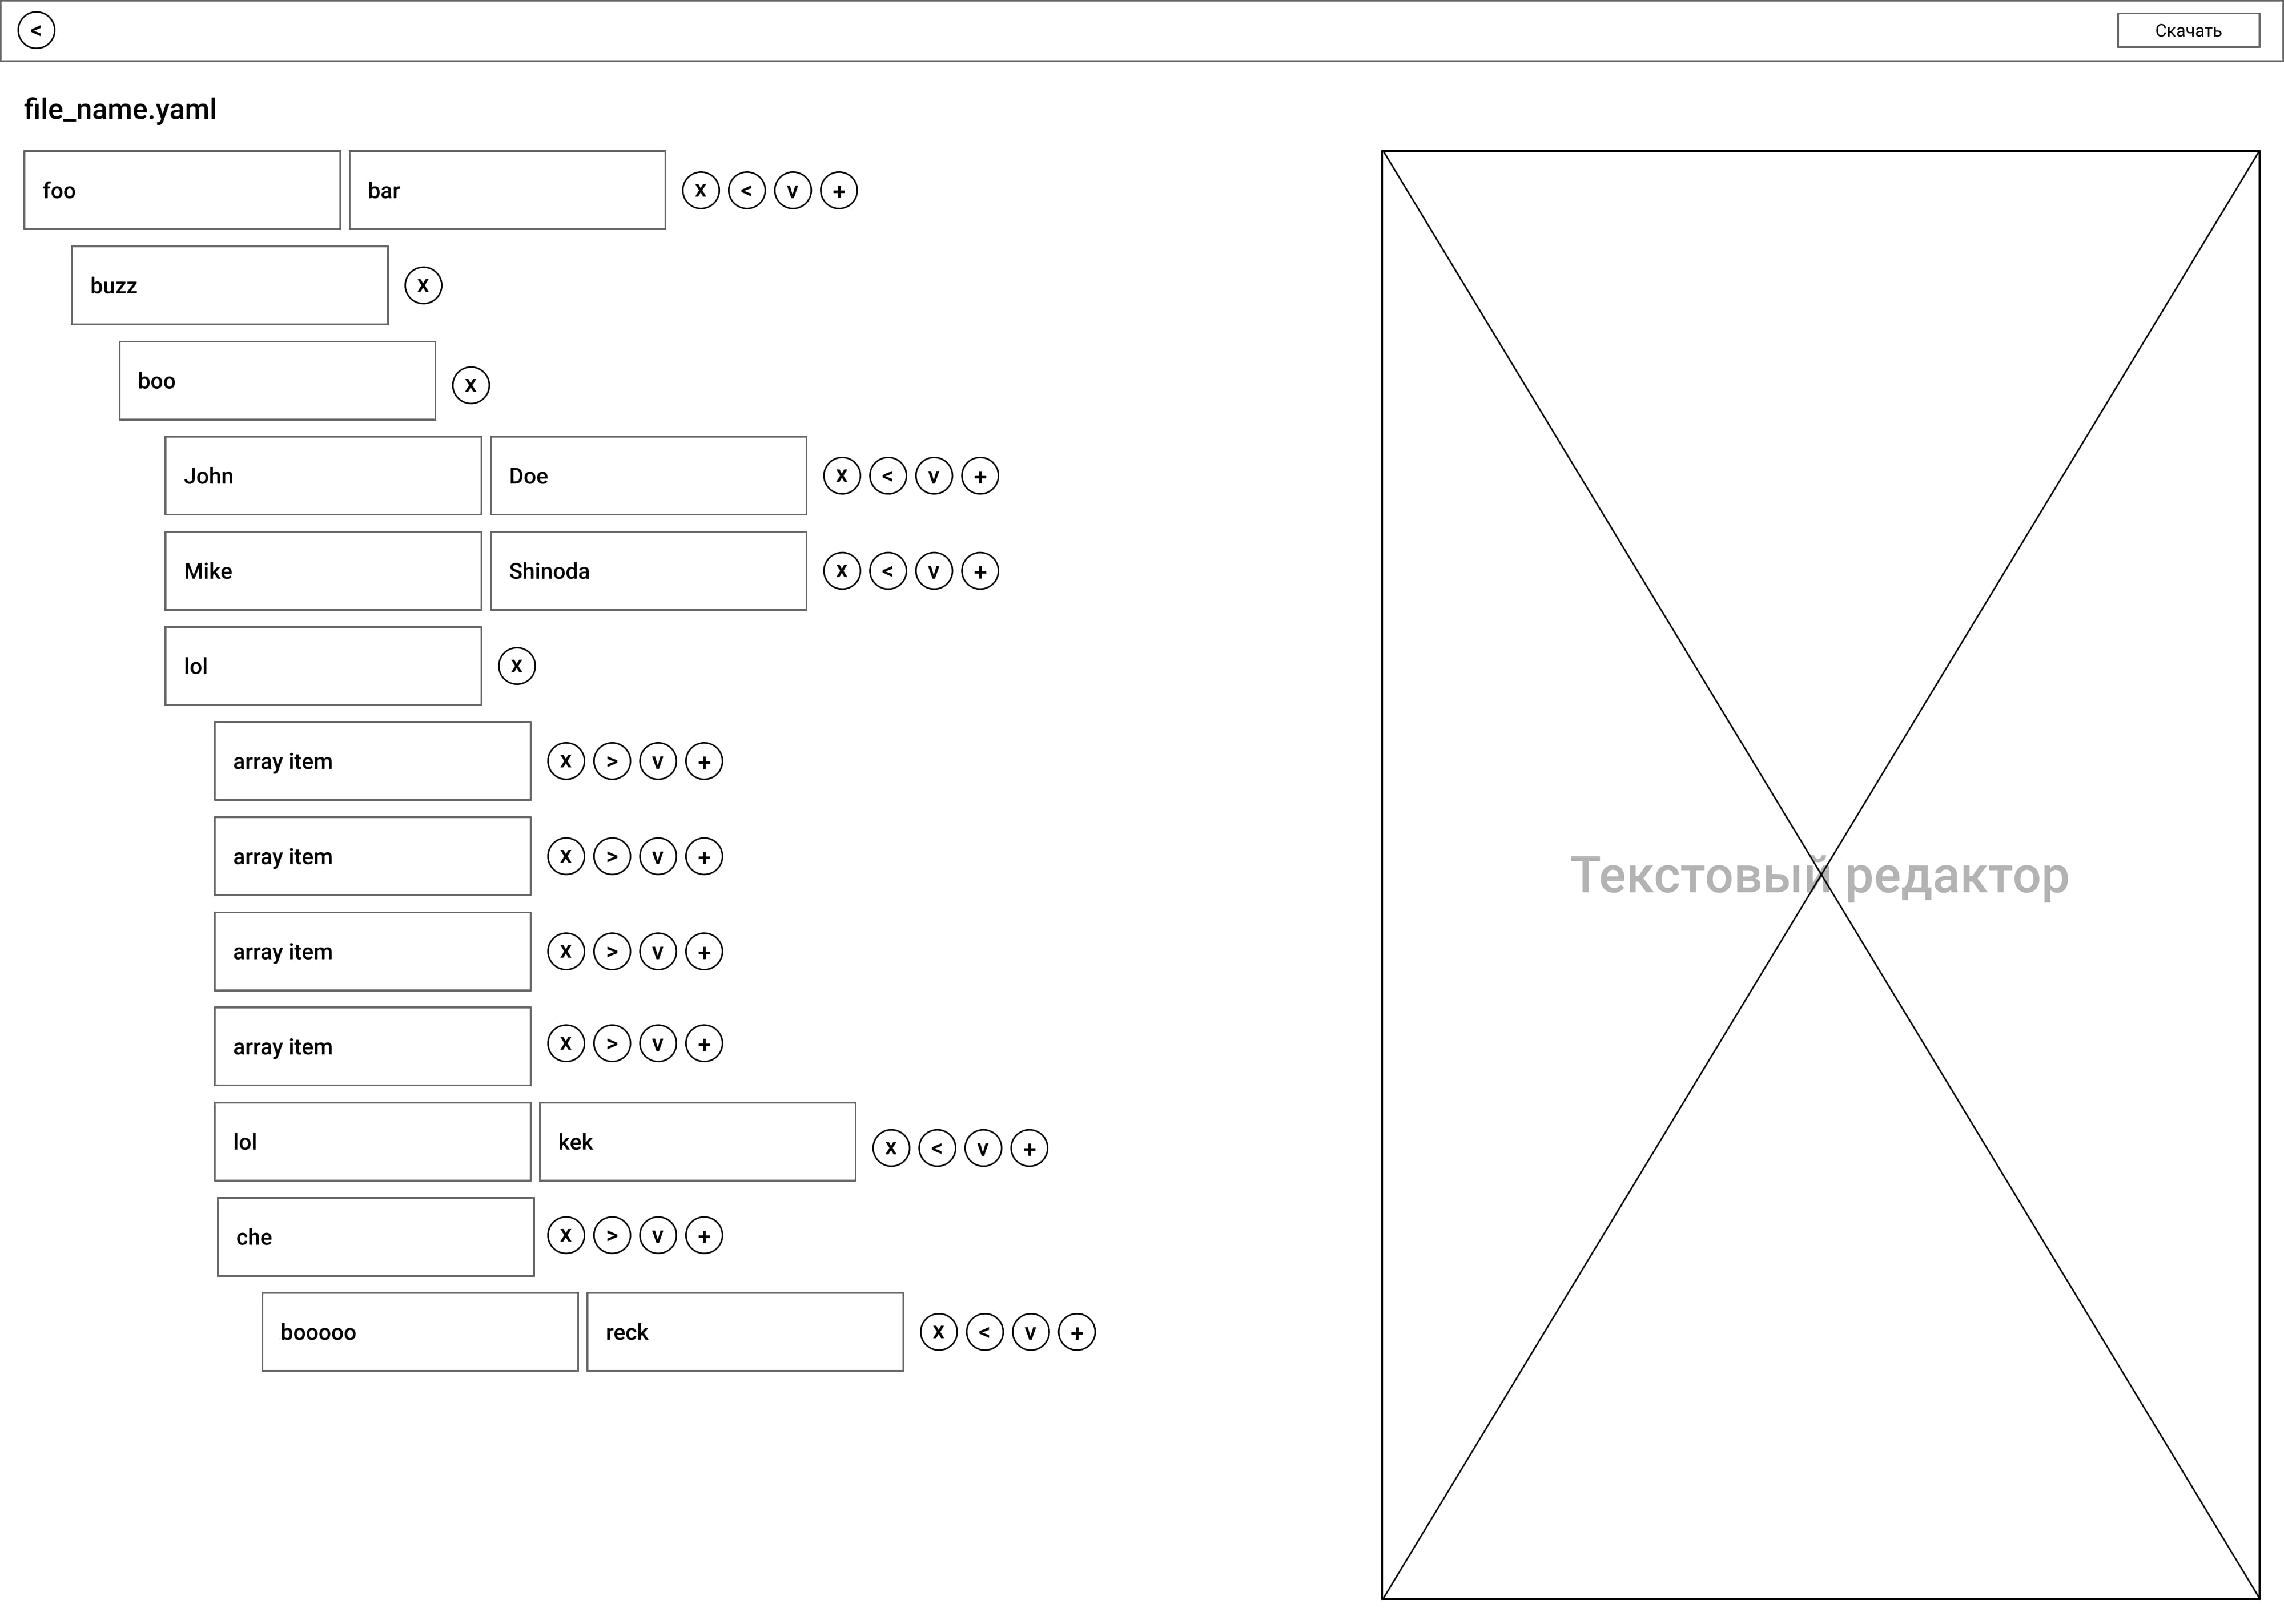
\includegraphics[scale=0.09]{Editor (visitor).jpg}}
    \caption{Прототип дизайна редактора, если пользователь имеет статус посетителя}
    \label{des:proto_3}
\end{figure}

\begin{figure}[H]
    \center{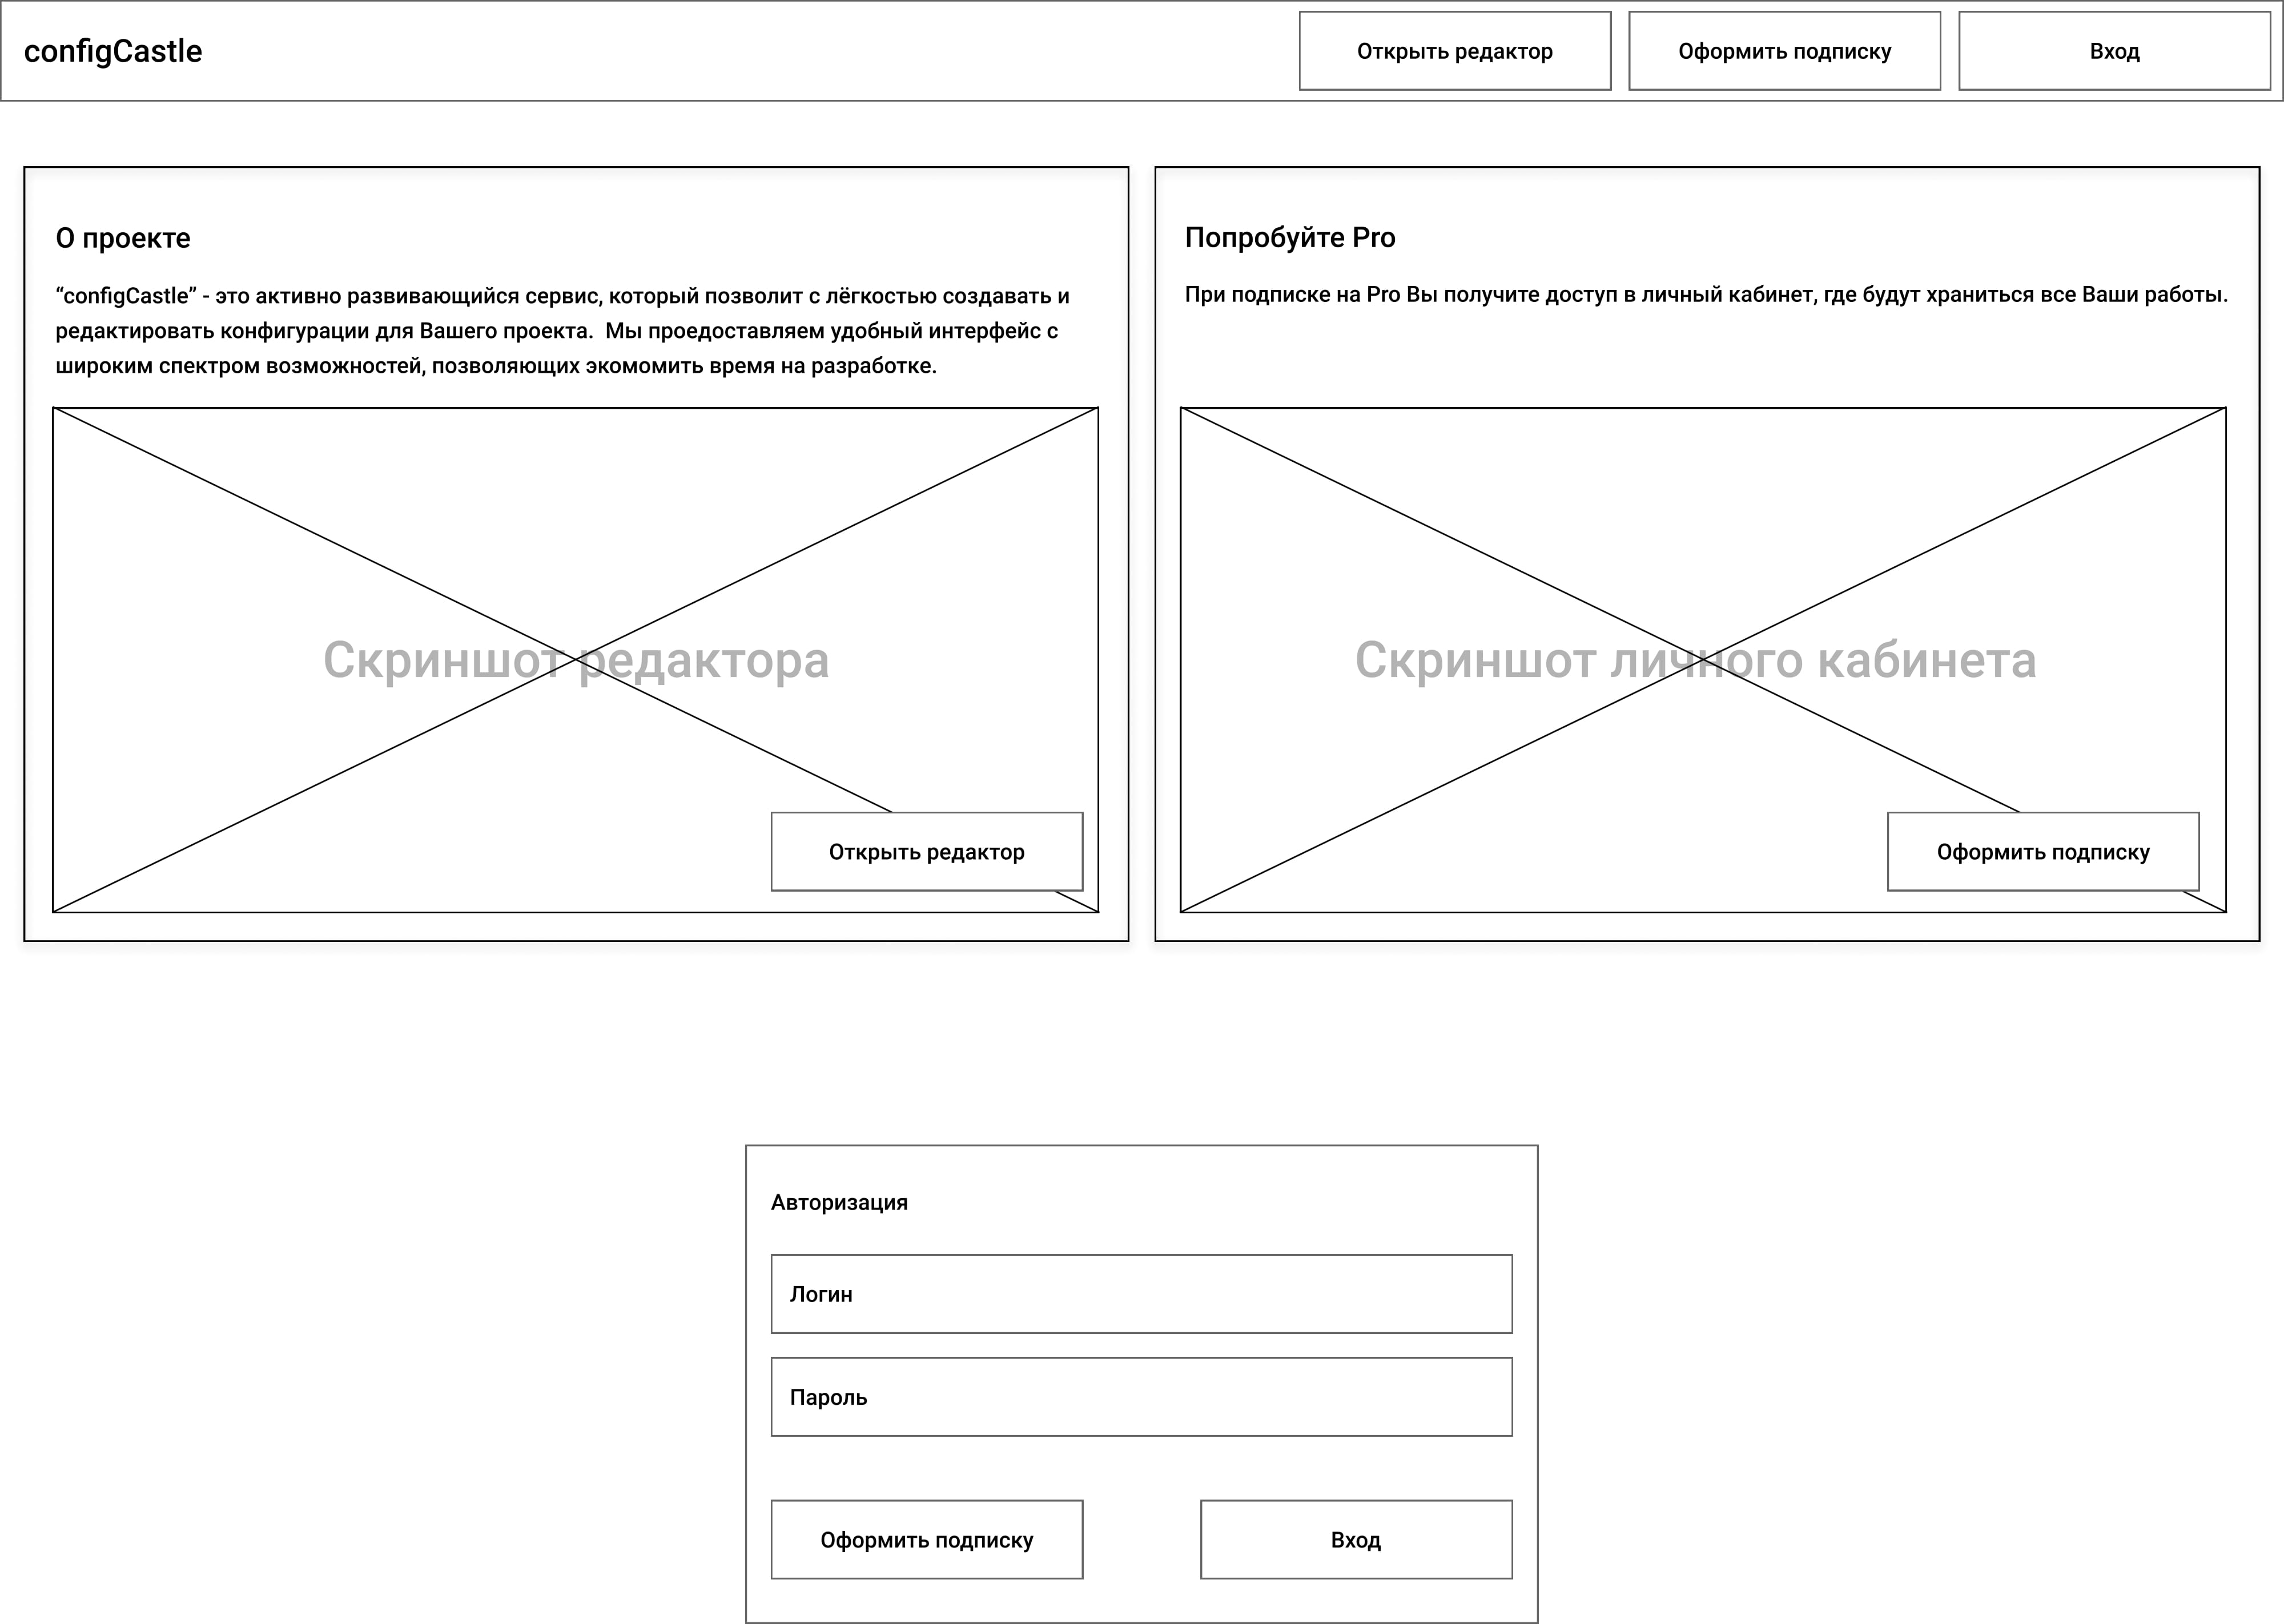
\includegraphics[scale=0.09]{Title (log in).jpg}}
    \caption{Прототип страницы с возможностью входа}
    \label{des:proto_4}
\end{figure}

\begin{figure}[H]
    \center{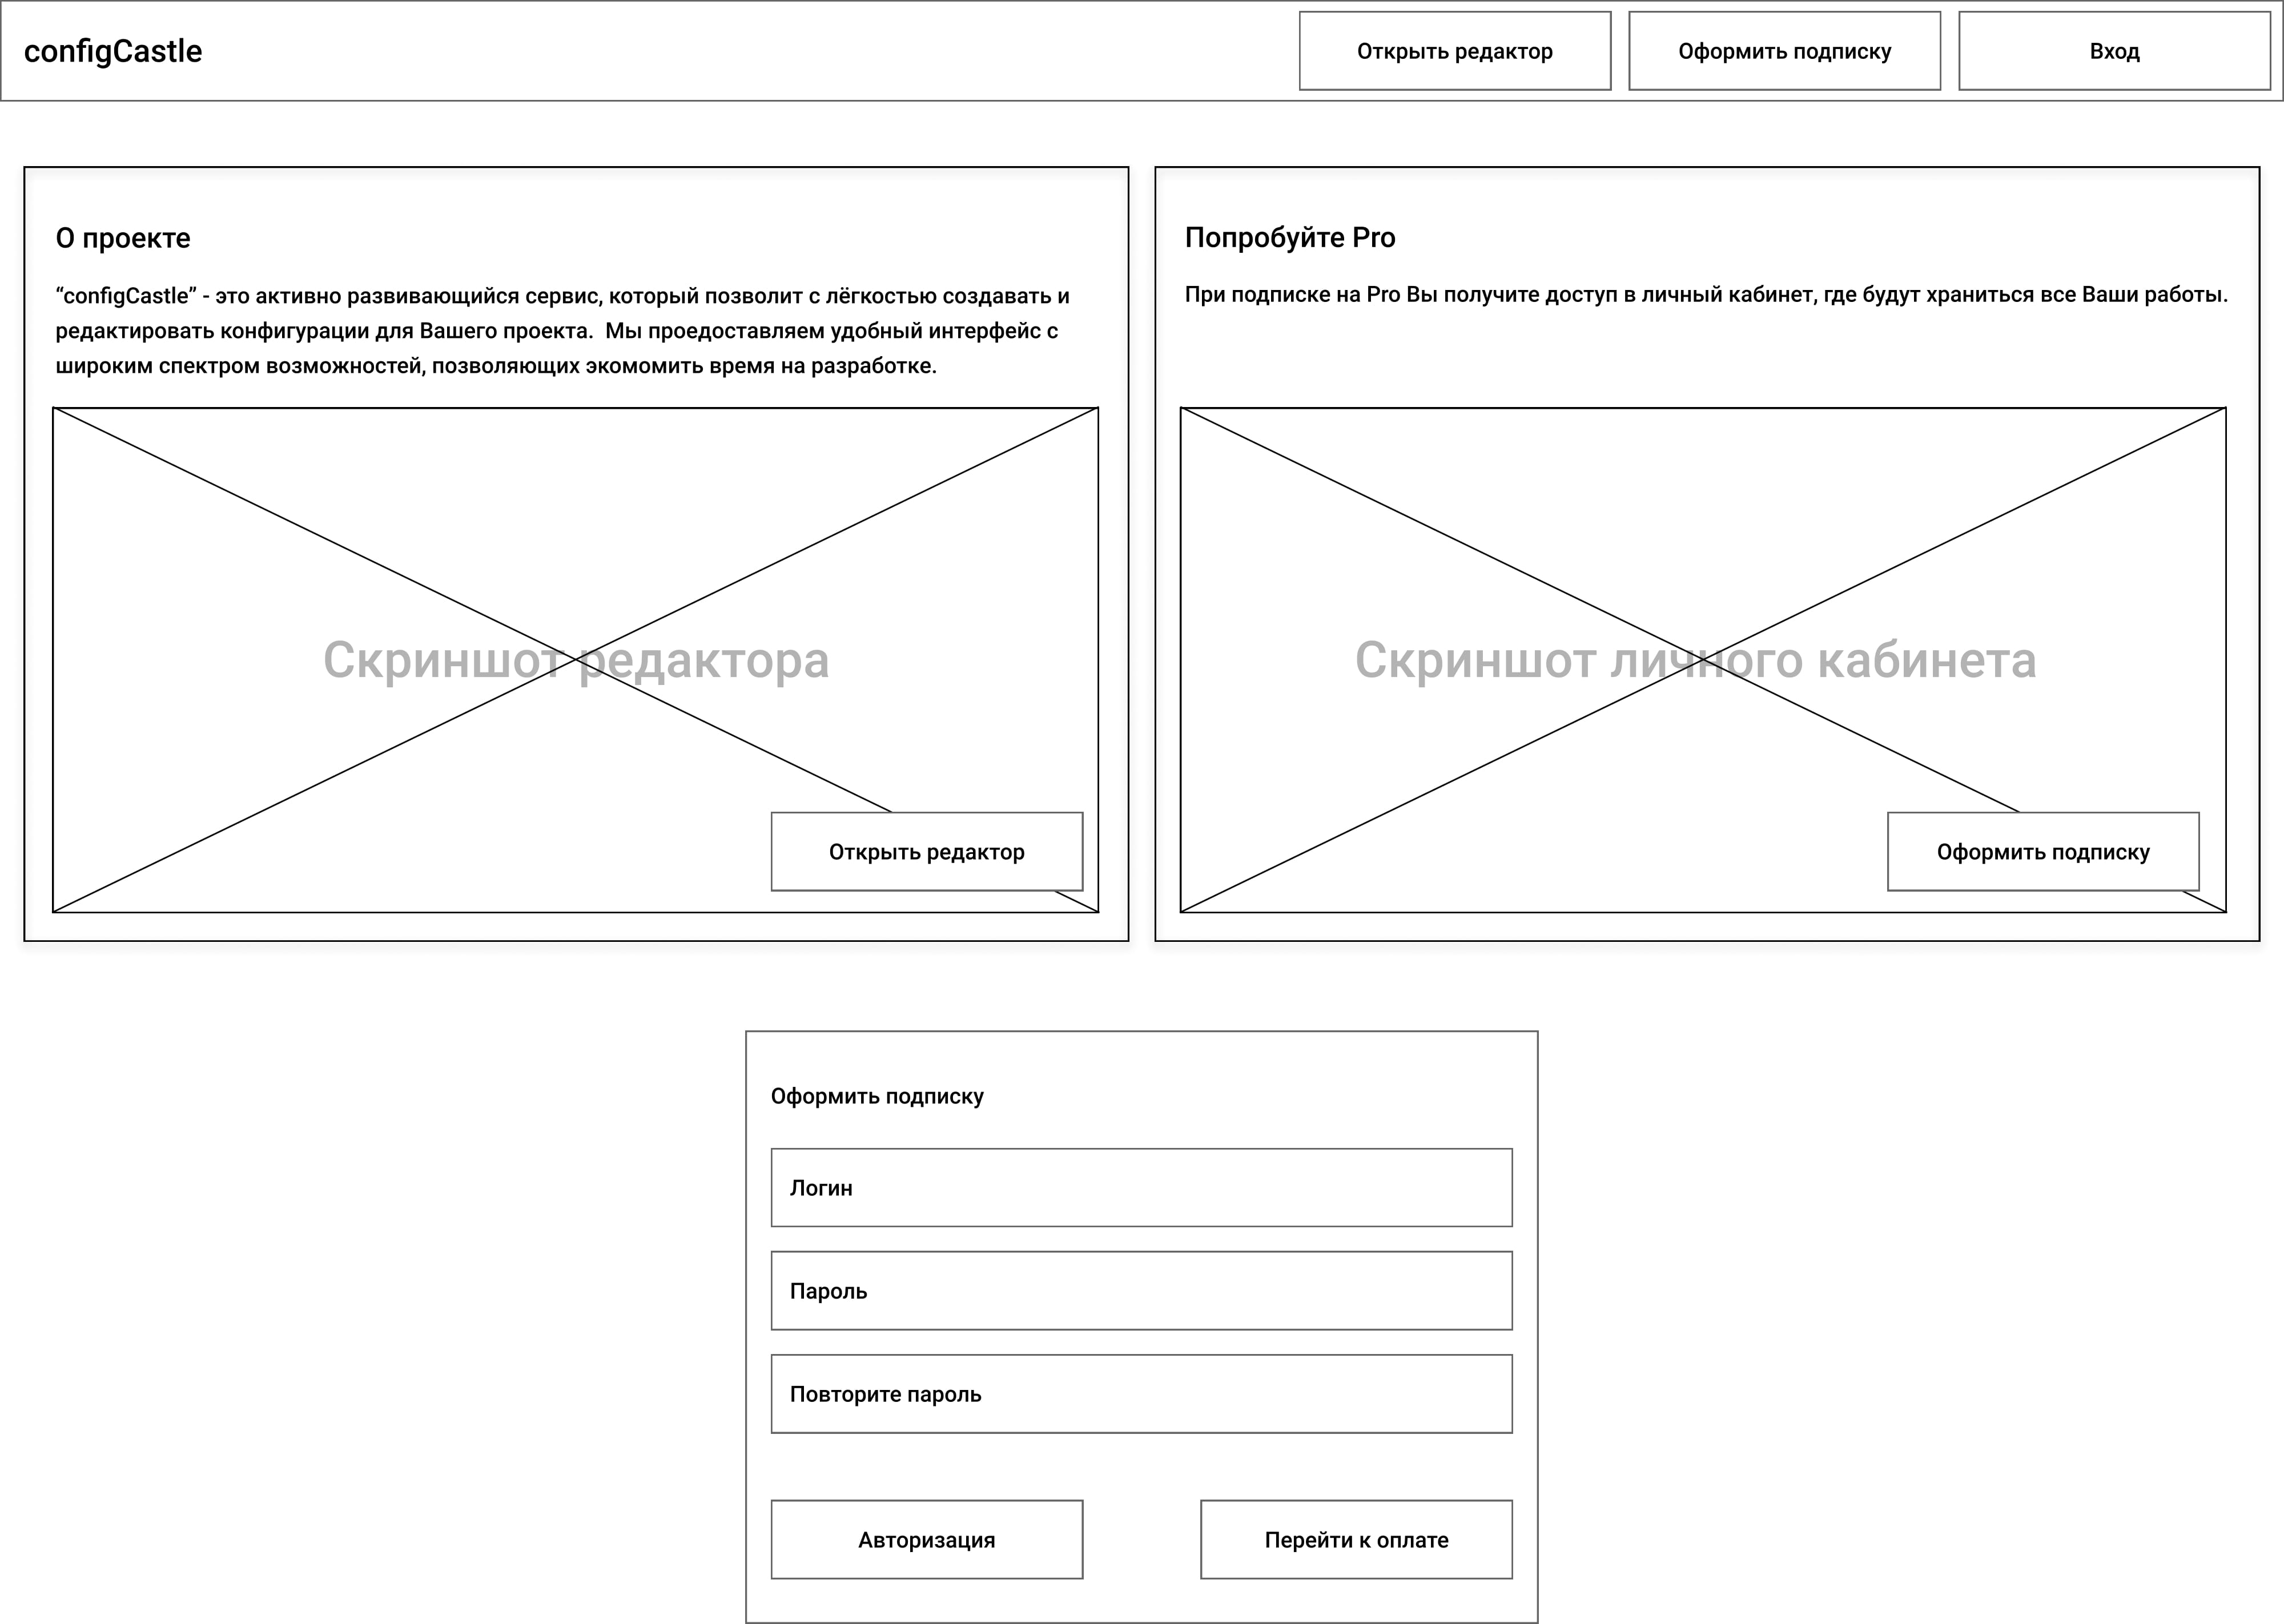
\includegraphics[scale=0.09]{Title (sign in).jpg}}
    \caption{Прототип страницы с возможностю создать аккаунт}
    \label{des:proto_5}
\end{figure}

\begin{figure}[H]
    \center{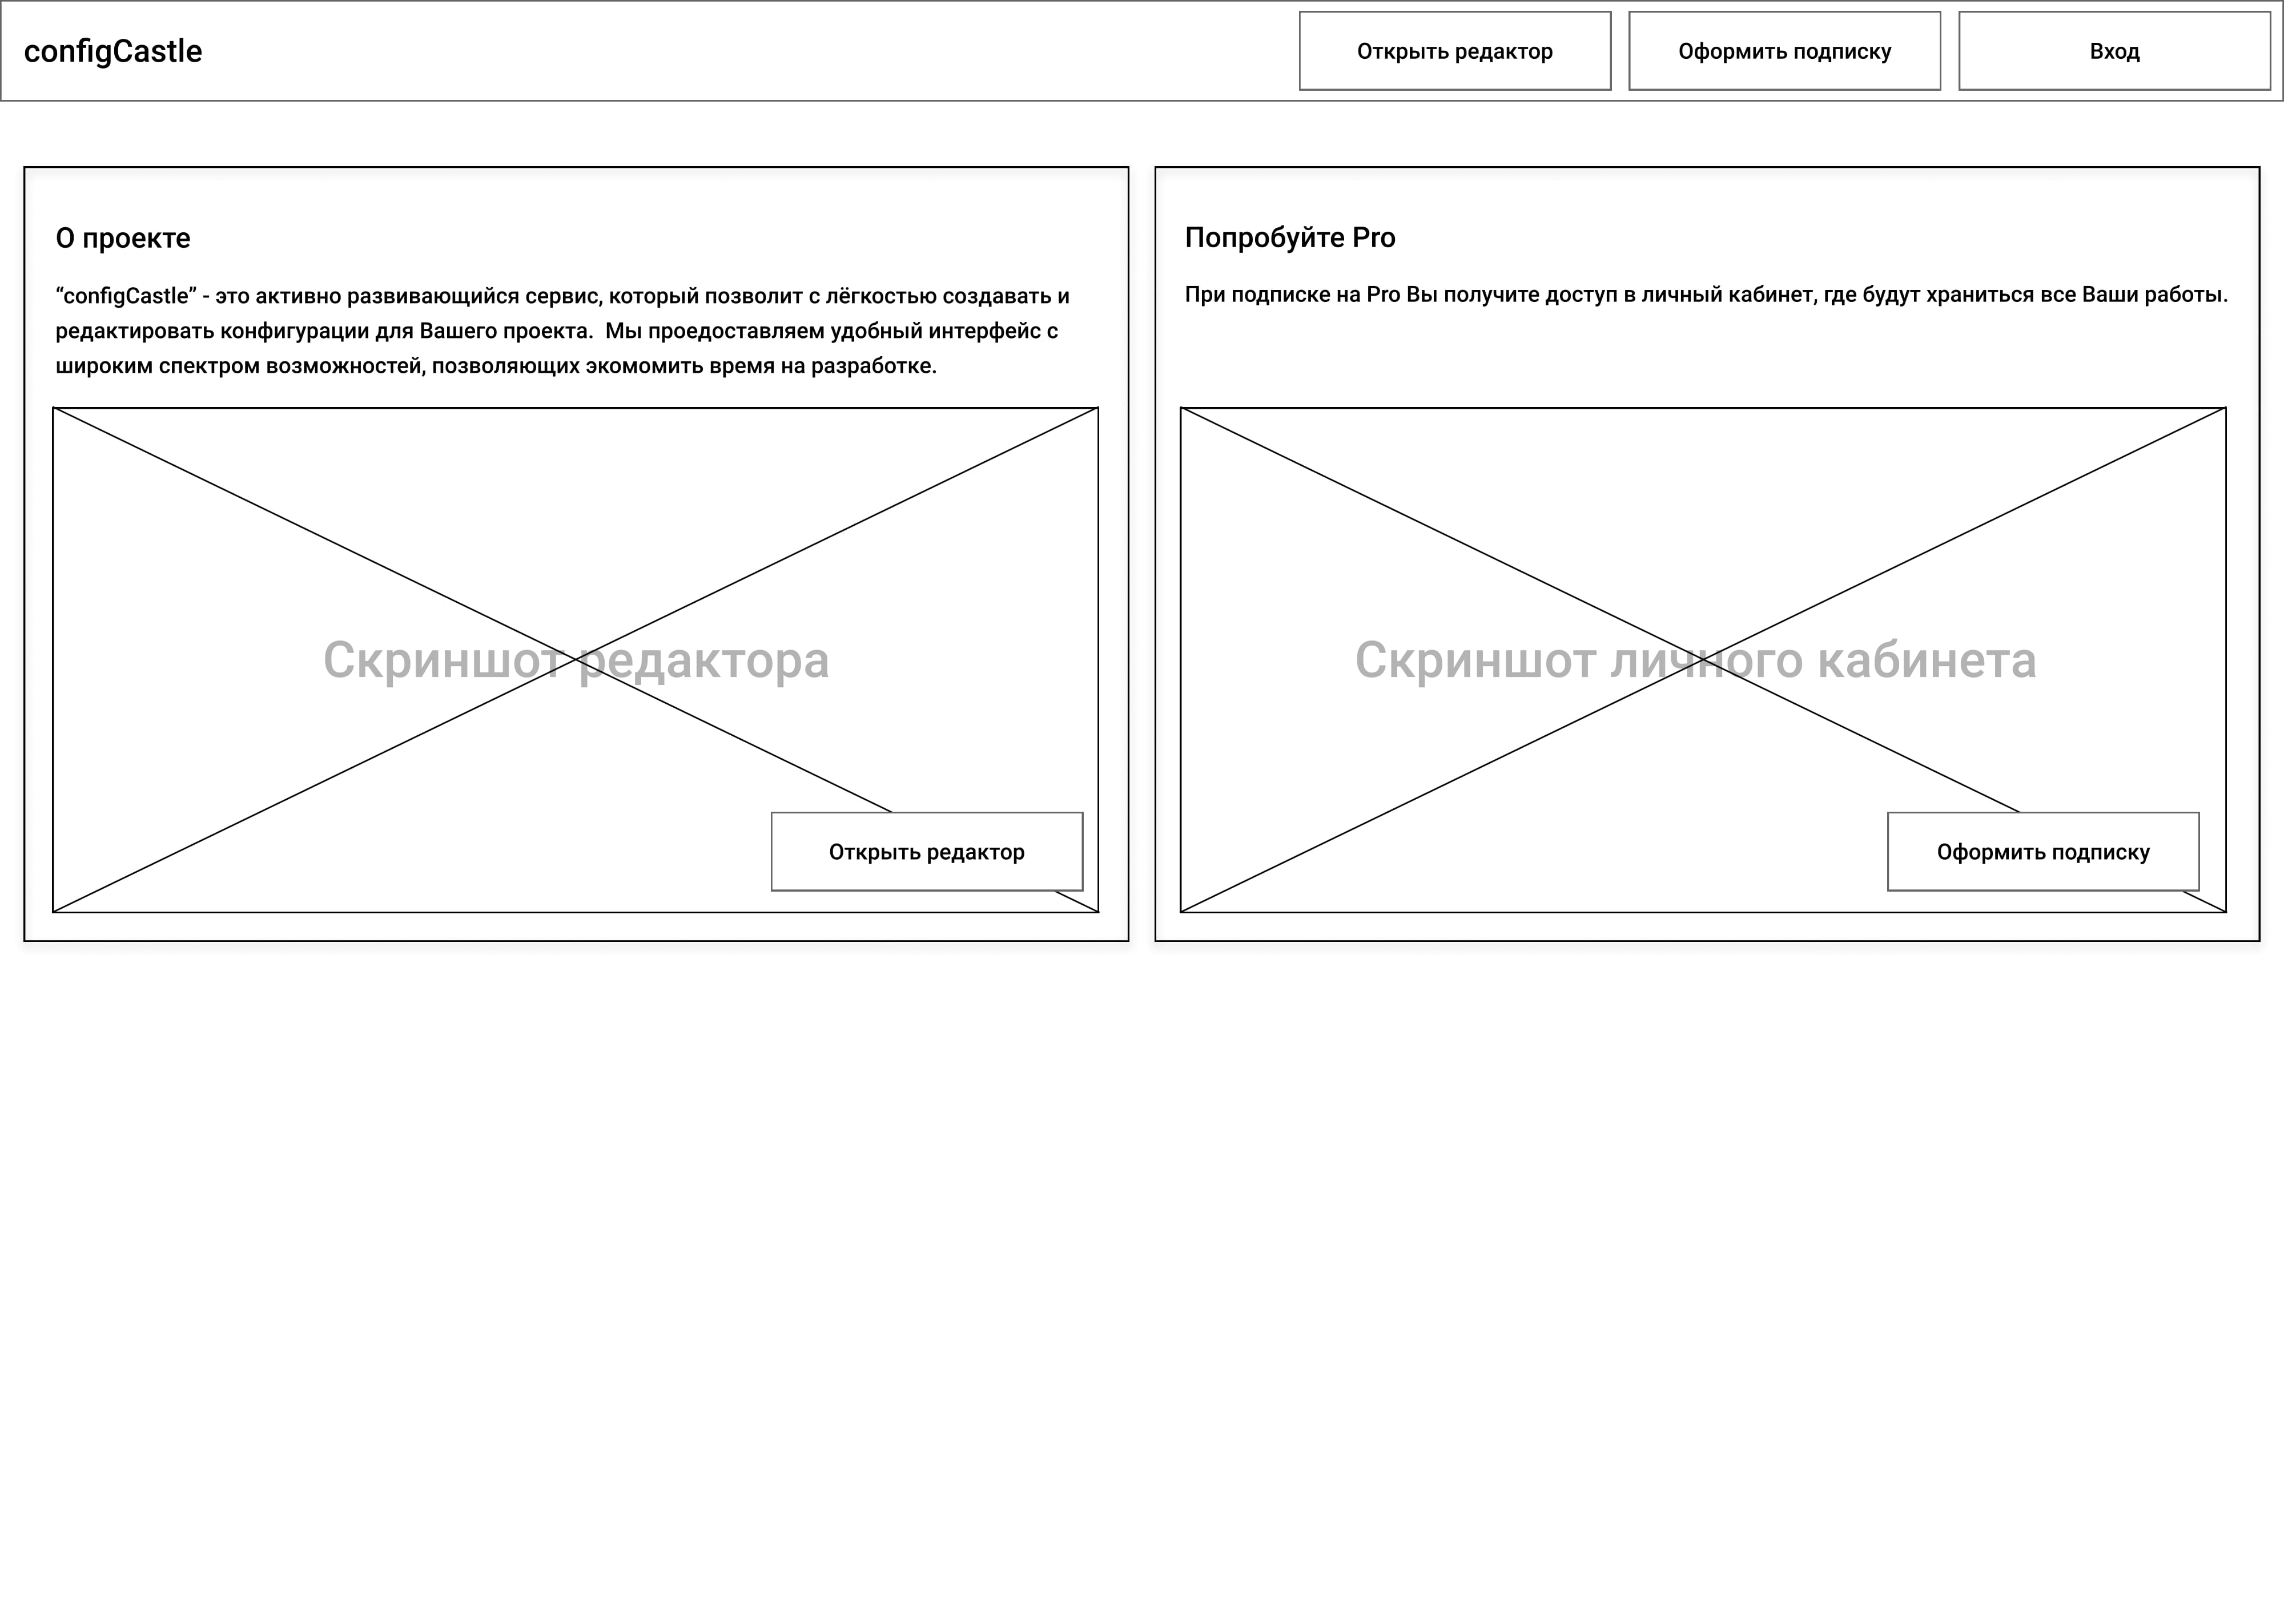
\includegraphics[scale=0.09]{Title.jpg}}
    \caption{Протип заглавной страницы}
    \label{des:proto_6}
\end{figure}

\subsection{Архитектура программного продукта}

В ходе проектирования определённое время заняло разработка архитектура и планирование общего взаимодействия компонентов приложений.

Архитектура программного продукта представляет из себя простой клиент-сервер. Только в этом в этом случае имеется два необщающися между собой сервера, но имеющие
доступ к одной базе данных, описываемой в разделе \ref{des:bd_section}.

В первую очередь, имеется клиентское приложение. Именно с ним будет взаимодейстовать пользователь: получать с помощью него свои данные, если таковые имеются,
работать с интерфейсом, вносить новые данные и так далее. Сам клиент взаимодействует с двумя серверными частями, которые являются отдельными друг от друга приложениями.

Сервер GraphQL представляет собой серверное приложение, которое необходимо для работы редактора. Оно регистрирует для этого роут и определяет типа для GraphQL, предоставлля
Query и Mutation, которое затем может выполнять и отправлять серверу в виде JSON. Работает непосредственно с базой данной, используя специализированный для этого драйвер.

Сервер авторизации и аутенфикации создан для работы с пользователем. Это приложение не знает о сервере GraphQL, работая независимо, но с той же базой данных, используяя
RESTfulll API.

База данных хранит информацию о пользователя, созданных файлах и сервисах и нужна для постоянной работы приложения.

Схематично архитектура программного продукта отображена на рисунке \ref{des:arch}.

\begin{figure}[H]
    \center{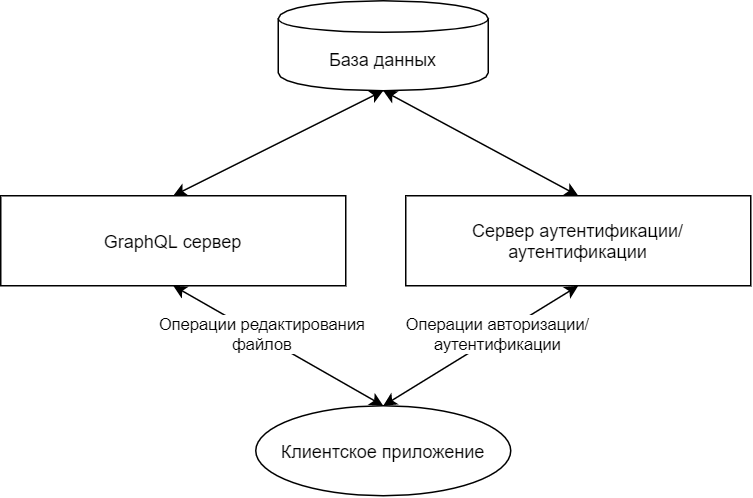
\includegraphics[scale=0.5]{arch.png}}
    \caption{Архитектура проекта}
    \label{des:arch}
\end{figure}

\subsection{Проектирование базы данных}

\label{des:bd_section}

В ходе проекторивания, выбор СУБД остановился на MongoDB. Она позволяет хранить неструктурированные данные в определённых коллекциях в виде JSON, делая работа с этим форматом удобнее.
Так как потенциально могут возникнуть сервисы с непостоянной структурой, то это делает серверное приложение масшатибируемым, не создаваяя множество миграций. Также для MondoDB имеется
хорошие драйвера, в том числе и асинхронные, что делает этот выбор ещё и производительнее.

Мы имеем определённое количество коллекций, присущих MongoDB ~--- file, service и user, которые хранят соответсвующие данные в виде документов, которые не подчиняются единой
структуре.

На рисунке \ref{des:bd_image} схематично описана структура базы данных.

\begin{figure}[H]
    \center{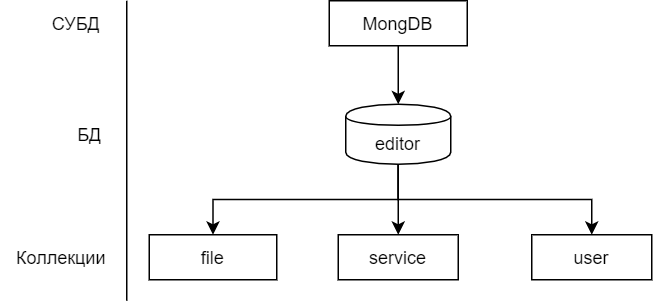
\includegraphics[scale=0.5]{bd.png}}
    \caption{Схематичное описание структуры базы данных}
    \label{des:bd_image}
\end{figure}

    \newpage
    \section{Разработка программного продукта}

На этапе подготвки к разработке программного продукта, необходимо выбрать соответсвующие целям средства для разработки, а также составить
график разработки, ориентируясь на него в процессе работы.

\subsection{Инструментальные и программные средства разработки}

Чтобы приступить к разработке необходимо выбрать такие средства как:

\begin{enumerate}
    \item язык программирования;
    \item система контроля версий;
    \item хостинг кода;
    \item библиотеку для серверной части;
    \item библиотеку для написания GraphQL-сервера;
    \item систему упаковки приложения;
    \item редактор кода.
\end{enumerate}

\subsubsection{Язык программирования}

После проектирования было необходимо выбрать нужные Инструментальные и программные средства разработки.

Так как темой дипломного проекта являлась написание серверной части, то выбор состоял из трёх языков программирования: PHP, JavaScript(Node.js) и Python.

Ниже привидено краткое сравнение языков программирования и затем будут сделаны соответсвующие выводы:

\paragraph{Необходимые библиотеки и фреймоворки}

PHP: Обладает многими
фреймворками, такими
Symfony, Laravel и так
далее.

Node.js: Создан в первую
очередь для 
написания
серверных 
приложений. Однако сущесвуют такие фреймоврки как Express и Nest.js, которые облегчают разработку.

Python: Python имеет в
своём распоряжении
множество библиотек,
которые работают как
синхронно, так 
и асинхронно. Например, Django и aiohttp.

\paragraph{Стиль кода}

PHP: На момент сравнения
не было найдено
единого стандарта кода.

Node.js: Не обладает таким
стандартом.

Python: имеет PEP-8.

\paragraph{Документирование}

PHP: Имеет phpDocumentator,
но не входит в стандарт.

Node.js: Не обладает 
средством
автоматического 
документирования.

Python: Имеет в распоряжении 
pydoc, входящий в 
стандарт, 
единый принцип 
Docstringsи обладает
множеством линтеров.

\paragraph{Стиль исполнения}

PHP: Создаёт объект
приложения на каждый
запрос.

Node.js: Запускает единый 
сервер, где 
разрешает 
каждый запрос
соответсвующей
функцией.

Python: Схож с Node.js при использовании бекенд-фреймворк.

\paragraph{Выводы}

Исходя из вышесказанного был выбран язык программирования Python. Так как он относительно легок синтаксически, схож с Node.js по стилю исполнения,
имеет средство автоматической документации и входящий в стандарт PEP-8, что повывашает единообразие кода и выбор линтеров.

\subsubsection{Система контроля версий}

Системой контроля версий был выбран git, так как он является де-факто стандартом индустрии, несмотря на некоторые технические преимущества Mercurial.
По этой же причине с ним знакомы большинство разработчиков, поддерживающих открытое программноое обеспечение, что сэкономит время и финансы, если в проект
придут новые люди.

\subsubsection{Средство хостинга кода}

Необходимо было выбрать средсто хранения кода, так как это позволило бы работать с разных устройств, обмениваться наработками и коммитами и так далее.
Так как средством контроля версий был выбран git, то выбор стоял между GitHub, GitLab и Bitbucket.

Сравнение будет идти только между сообществом и встроенными возможностью CI и CD. Такой пункт как интерфейс является субъективным и не учитывается
в процессе выбора средств.

\paragraph{Сообщество}

GitHub: обладает большим сообществом разработчиков, вкладывающих в открыте проекта. Большинство библиотек расположены в GitHub.

GitLab: сообщество меньше, а GitLab больше используется в корпоративных целях чему способствует возможность распложить его на собственном сервере, иными словами
self-hosted.

Bitbucket: сообщество не развито, несмотря на что был одним из первых хостингов кода, работая изначально с Mercurial.

\paragraph{Возможности CI и CD}

GitHub: имеет простой и понятный, и бесплатный GitHub Actions. Семантически описывается в yaml файле; по синтаксису схож с docker-compose

GitLab: также имеет встроенный CI и CD, но в отлчии от GitHub Actions синтаксис простым назвать довольно трудно.

Bitbucket: тоже имеет CI/CD, однако бесплатные минуты значительно меньше, чем у GitHub.

\paragraph{Выводы}

Исходя из сравнения, выбор остановился на GitHub, так как он известен в сообщетсве открытого программного обеспечения, каковым является и configCastle и обладает встроенным
GitHub Actions, позволяющий автоматизировать рутинные задачи по запуску тестов после коммита.

\subsubsection{Библиотека для написания серверной части}

Исходя из требования к асинхронности программного продукта такие библиотеки как Django и Flask не рассматривались. Они работают в синхронном режиме, блокируя операции
ввода-вывода, а следовательно не подходят.

Одним из немногих кандидатов остался aiohttp, являющимся микро-фреймворком и работающем на встроенной библиотеке asyncio.

У aiohttp есть такие конкрунты как Sanic и FastAPI, однако количество дополнительных библиотек у них ограничено и сообщество не развито в достаточной мере.

\subsubsection{Библиотека для написания GraphQL-сервера}

Для того, чтобы реализовать GraphQL-сервер на Python можно воспользоваться двумя библиотеками:

\begin{itemize}
    \item Graphene;
    \item Tartiflette.
\end{itemize}

Был выбран Tartiflette, так как он:

\begin{itemize}
    \item асинхронный;
    \item работает с aiohttp;
    \item понимает язык sdl(schema definition language), являющимся родным для GraphQL.
\end{itemize}

\subsubsection{Система упаковки приложения}

Для того, чтобы доставлять код, библиотеки и прочие зависимости в удобном виде каждому человеку, не нарушая уже сложившуюся экосистему, сущесвует
два способа:

\begin{itemize}
    \item Виртуальные машины;
    \item Docker;
\end{itemize}

Виртуальные машины эмулируют работу железа и потребляют много ресурсов устройства, однако способны полностью воспроизводить ОС. Такое излишество неудобно, поэтому был выбран
Docker.

Docker ~--- это система виртуализации на основе хостовой операционной системы. Работает с такими терминами как образ и контейнер. В контейнер можно упаковать код и его зависимости, а затем
доставить этот контейнер в виде образа любому другому человеку или хостингу.

\subsection{Редактор кода}

В основном, используются специализированные редакторы кода, такие как vim, emacs, visual studio code, atom, sublime text и так далее.

В процессе разработки были выбраны такие редакторы как vim для быстрого написания непродолжительных участков кода, так как:

\begin{itemize}
    \item быстр;
    \item очень прост;
    \item позволяет очень быстро исправлять ошибки за счет своего управления.
\end{itemize}

Visual Studio Code был выбран потому что:

\begin{itemize}
    \item обладает большим колчеством расширений, так в работе использовалось расширение Docker, позволяющее управлять всей экосистемой прямо в редакторе;
    \item удобная система конфигурации настроек проекта, например, подключение линтера, в виде файла settings.json, который нужно расположить в отдельном каталоге.
\end{itemize}

\subsection{Календарный план разработки продукта}

В процессе проектирования был составлен предполагаемый график разработки проекта, представленный в таблице \ref{dev:date}.

\begin{longtable}[c]{|l|l|l|}
    \caption{План разработки продукта}
    \label{dev:date}\\
    \hline
    Этап работы                                      & Начало   & Окончание \\ \hline
    \endfirsthead
    %
    \multicolumn{3}{c}%
    {{\bfseries Table \thetable\ continued from previous page}} \\
    \endhead
    %
    Разработка требований                            & 01.11.19 & 15.11.19  \\ \hline
    Создание прототипов пользовательского интерфейса & 18.11.19 & 22.11.19  \\ \hline
    Написание прототипа сервера                      & 21.11.19 & 28.11.19  \\ \hline
    Создание дизайна                                 & 24.11.19 & 30.11.19  \\ \hline
    Разработка общей архитектуры проекта             & 01.12.19 & 13.12.19  \\ \hline
    Выбор технологий                                 & 15.12.19 & 20.12.19  \\ \hline
    Изучение документации к выбранным технологиям    & 21.12.19 & 25.12.19  \\ \hline
    Написание кода клиентской части                  & 24.12.19 & 17.04.20  \\ \hline
    Написание кода серверной части                   & 19.01.20 & 16.04.20  \\ \hline
    Тестирование клиентской части                    & 18.04.20 & 24.04.20  \\ \hline
    Тестирование серверной части                     & 22.04.20 & 25.04.20  \\ \hline
    Развёртывание на сервере                         & 26.04.20 & 29.04.20  \\ \hline
\end{longtable}

После составления графика была создана диаграмма Ганта, исходя из данных представленных в таблице \ref{dev:date}. Эта диаграмма показана на рисунке \ref{dev:gant_image}.

\begin{figure}[H]
    \center{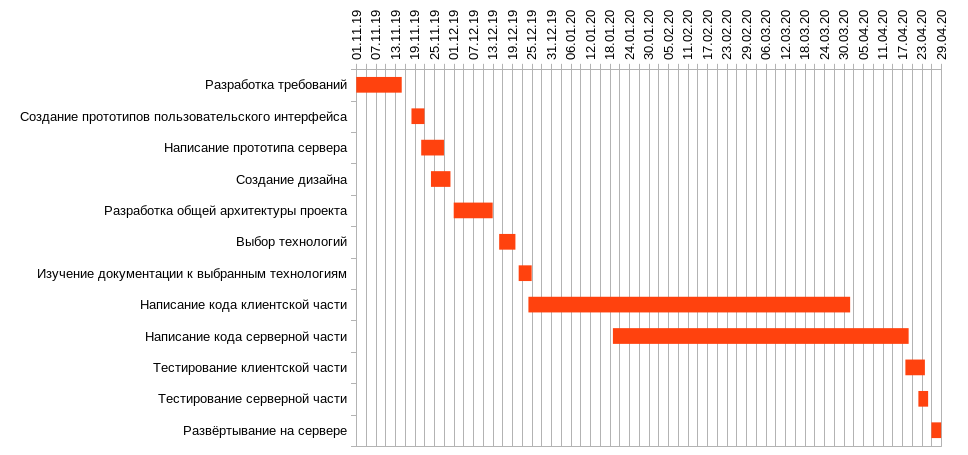
\includegraphics[scale=0.5]{gant.png}}
    \caption{Диаграмма Ганта}
    \label{dev:gant_image}
\end{figure}

    \newpage
    \section{Тестирование программного продукта}

Тестирование любого программного продукта необходимо, так как позволяет выявлять ошибки и получать обратную связь от пользователей и/или тестировщиков.
Для наиболее эффективного процесса тестирования выбираются оптимальные способы тестирования, а затем создаются тест-кейсы под уже выбранные методы.

\subsection{Выбор метода обеспечения качества}

Исходя из требований к тестированию необходимо провести его двумя способами:

\begin{enumerate}
    \item создать необходимые автоматические тесты;
    \item вручную протестировать результат работы GraphQL-сервера, созданного в процессе работы.
\end{enumerate}

\subsection{План тестирования}

Требуется провести тестирование работоспособности и качество
реализации проекта «configCastle». В рамках плана следует перечислить
программные составляющие и отдельные составляющие их функционала,
подлежащие оценке качества, подходы и виды тестирования, используемые в
данном процессе и график тестирования.

\subsubsection{Программные составляющие, подлежающие тестированию}

Следует провести тестирование следующих составляющих приложения:

\begin{itemize}
    \item возможность приложения работать базы данных, то есть записывать и получать данные;
    \item ответы GraphQL-сервера, предусмотренных техническим заданием, используя окружение GraphiQL.
\end{itemize}

Автотесты исполняются с помощью системы pytest\_aiohttp, используя экосистему py.test.

\subsubsection{Тест-план}

Для корретного тестирования необходимо составить тест-план с где можно отслеживать какие именно тесты необходимо провести, чтобы
убедиться в работоспобности приложения. Тест-план представлен в таблице \ref{dev:test_plan}.

\begin{longtable}[c]{|l|l|}
    \caption{Тест-план}
    \label{dev:test_plan}\\
    \hline
    Идентификатор & Название тесты \\ \hline
    \endfirsthead
    %
    \multicolumn{2}{c}%
    {{\bfseries Table \thetable\ continued from previous page}} \\
    \hline
    Идентификатор & Название тесты \\ \hline
    \endhead
    %
    1             &      Проверка query service(id: \textless{}Number\textgreater{})          \\ \hline
    2             &      Проверка query services          \\ \hline
    3             &      Проверка query file(id: \textless{}Number\textgreater{})          \\ \hline
    4             &      Проверка query files          \\ \hline
    5             &      Проверка mutation createFile          \\ \hline
    6             &      Проверка mutation updateFile          \\ \hline
    7             &      Првоерка mutation deleteFile         \\ \hline
    8             &      Обновление файла с несуществующим id          \\ \hline
\end{longtable}

\subsubsection{Тест-кейсы}

Для правильного тестирования были составлены подробные тест-кейсы или сценария тестирования, описывающий процесс тестирования
каждого созданного запроса. Данные сценарии представлены в таблицах \ref{test:case_1}, \ref{test:case_2}, \ref{test:case_3}, \ref{test:case_4},
\ref{test:case_5}, \ref{test:case_6}, \ref{test:case_7}, \ref{test:case_8}.

\begin{longtable}[c]{|l|l|}
    \caption{Тест-кейс №1}
    \label{test:case_1}\\
    \hline
    Идентификатор & 1                                                                                                \\ \hline
    \endfirsthead
    %
    \multicolumn{2}{l}%
    {{Продолжение таблицы \thetable \vspace{0.5cm}}} \\
    \hline
    \endhead
    %
    Название                            & Проверка query service(id: \textless{}Number\textgreater{})                                                            \\ \hline
    Приоритет                           & Высокий                                                                                                               \\ \hline
    Дата проведения                     & 22.04.2020                                                                                                            \\ \hline
    Описание                            & \begin{tabular}[c]{@{}l@{}}Тестируется правильность возвращения\\ данных при использовании query service\end{tabular} \\ \hline
    Предусловие                         & Отсутствует                                                                                                           \\
    \pagebreak
    Шаги тестирования &
      \begin{tabular}[c]{@{}l@{}}1) Запустить graphiQL проекта;\\ 2) Использовать следующий запрос:\\      query \{\\           \hspace{2ex}service(id: 1) \{\\                 \hspace{4ex}name\\                 \hspace{4ex}id\\                 \hspace{4ex}data\\           \hspace{2ex}\}\\      \}\end{tabular} \\ \hline
    Ожидаемый результат                 & \begin{tabular}[c]{@{}l@{}}Появление полей в виде ответа по структуре\\ совпадающих с запросом\end{tabular}           \\ \hline
    Постусловие                         & Отсутсвует                                                                                                            \\ \hline
    Фактический результат               & Совпадает с ожидаемым                                                                                                 \\ \hline
    Статус                              & Пройден                                                                                                               \\ \hline
\end{longtable}

\begin{longtable}[c]{|l|l|}
    \caption{Тест-кейс №2}
    \label{test:case_2}\\
    \hline
    Идентификатор & 2                                                                                                \\ \hline
    \endfirsthead
    %
    \multicolumn{2}{l}%
    {{Продолжение таблицы \thetable \vspace{0.5cm}}} \\
    \hline
    \endhead
    %
    Название                            & Проверка query services                                                            \\
    Приоритет                           & Высокий                                                                                                               \\ \hline
    Дата проведения                     & 22.04.2020                                                                                                            \\ \hline
    Описание                            & \begin{tabular}[c]{@{}l@{}}Тестируется правильность возвращения\\ данных при использовании query services\end{tabular} \\ \hline
    Предусловие                         & Отсутствует                                                                                                           \\ \hline
    Шаги тестирования &
      \begin{tabular}[c]{@{}l@{}}1) Запустить graphiQL проекта;\\ 2) Использовать следующий запрос:\\      query \{\\           \hspace{2ex}services\{\\                 \hspace{4ex}name\\                 \hspace{4ex}data\\           \hspace{2ex}\}\\      \}\end{tabular} \\
    \pagebreak
    Ожидаемый результат                 & \begin{tabular}[c]{@{}l@{}}Появление полей в виде ответа по структуре\\ совпадающих с запросом\end{tabular}           \\ \hline
    Постусловие                         & Отсутсвует                                                                                                            \\ \hline
    Фактический результат               & Совпадает с ожидаемым                                                                                                 \\ \hline
    Статус                              & Пройден                                                                                                               \\ \hline
\end{longtable}

\begin{longtable}[c]{|l|l|}
    \caption{Тест-кейс №3}
    \label{test:case_3}\\
    \hline
    Идентификатор & 3                                                                                                \\ \hline
    \endfirsthead
    %
    \multicolumn{2}{l}%
    {{Продолжение таблицы \thetable \vspace{0.5cm}}} \\
    \hline
    \endhead
    %
    Название                            & Проверка query file(id: \textless{}Number\textgreater{})                                                            \\ \hline
    Приоритет                           & Высокий                                                                                                               \\ \hline
    Дата проведения                     & 22.04.2020                                                                                                            \\ \hline
    Описание                            & \begin{tabular}[c]{@{}l@{}}Тестируется правильность возвращения\\ данных при использовании query file\end{tabular} \\ \hline
    Предусловие                         & Отсутствует                                                                                                           \\
    Шаги тестирования &
      \begin{tabular}[c]{@{}l@{}}1) Запустить graphiQL проекта;\\ 2) Использовать следующий запрос:\\      query \{\\           \hspace{2ex}file(id: 1)\{\\                 \hspace{4ex}name\\                 \hspace{4ex}id\\                 \hspace{4ex}data\\           \hspace{2ex}\}\\      \}\end{tabular} \\ \hline
    Ожидаемый результат                 & \begin{tabular}[c]{@{}l@{}}Появление полей в виде ответа по структуре\\ совпадающих с запросом\end{tabular}           \\ \hline
    Постусловие                         & Отсутсвует                                                                                                            \\ \hline
    Фактический результат               & Совпадает с ожидаемым                                                                                                 \\ \hline
    Статус                              & Пройден                                                                                                               \\ \hline
\end{longtable}

\begin{longtable}[c]{|l|l|}
    \caption{Тест-кейс №4}
    \label{test:case_4}\\
    \hline
    Идентификатор & 4                                                                                               \\ \hline
    \endfirsthead
    %
    \multicolumn{2}{l}%
    {{Продолжение таблицы \thetable \vspace{0.5cm}}} \\
    \hline
    \endhead
    %
    Название                            & Проверка query files                                                         \\ \hline
    Приоритет                           & Высокий                                                                                                               \\ \hline
    Дата проведения                     & 23.04.2020                                                                                                            \\ \hline
    Описание                            & \begin{tabular}[c]{@{}l@{}}Тестируется правильность возвращения\\ данных при использовании query files\end{tabular} \\ \hline
    Предусловие                         & Отсутствует                                                                                                           \\ \hline
    Шаги тестирования &
      \begin{tabular}[c]{@{}l@{}}1) Запустить graphiQL проекта;\\ 2) Использовать следующий запрос:\\      query \{\\           \hspace{2ex}files\{\\                 \hspace{4ex}name\\                               \hspace{4ex}data\\           \hspace{2ex}\}\\      \}\end{tabular} \\ \hline
    Ожидаемый результат                 & \begin{tabular}[c]{@{}l@{}}Появление полей в виде ответа по структуре\\ совпадающих с запросом\end{tabular}           \\ \hline
    Постусловие                         & Отсутсвует                                                                                                            \\ \hline
    Фактический результат               & Совпадает с ожидаемым                                                                                                 \\ \hline
    Статус                              & Пройден                                                                                                               \\ \hline
\end{longtable}

\begin{longtable}[c]{|l|l|}
    \caption{Тест-кейс №5}
    \label{test:case_5}\\
    \hline
    Идентификатор & 5                                                                                                \\ \hline
    \endfirsthead
    %
    \multicolumn{2}{l}%
    {{Продолжение таблицы \thetable \vspace{0.5cm}}} \\
    \hline
    \endhead
    %
    Название                            & Проверка mutation createFile                                                           \\ \hline
    Приоритет                           & Высокий                                                                                                               \\ \hline
    Дата проведения                     & 23.04.2020                                                                                                            \\ \hline
    Описание                            & \begin{tabular}[c]{@{}l@{}}Тестируется правильность возвращения\\ данных при использовании query service\end{tabular} \\ \hline
    Предусловие                         & Отстуствие файлов в базе данных                                                                                                           \\
    Шаги тестирования &
      \begin{tabular}[c]{@{}l@{}}1) Запустить graphiQL проекта;\\ 2) Использовать следующий запрос:\\      mutation \{\\           \hspace{2ex}createFile\{input: \{\\ \hspace{6ex} data: \textquotedblleft\{\}\textquotedblright,\\ \hspace{6ex} name: `` test\_file'',\\ \hspace{6ex} configType: DOCKER\_COMPOSE, \\ \hspace{2ex}) \{\\                 \hspace{4ex}name\\                 \hspace{4ex}id\\                 \hspace{4ex}data\\           \hspace{2ex}\}\\      \}\end{tabular} \\ \hline
    Ожидаемый результат                 & \begin{tabular}[c]{@{}l@{}}Появление полей в виде ответа по структуре\\ совпадающих с запросом\end{tabular}           \\ \hline
    Постусловие                         & Отсутсвует                                                                                                            \\ \hline
    Фактический результат               & Файл создался с id 1                                                                                                 \\ \hline
    Статус                              & Провален                                                                                                               \\ \hline
\end{longtable}

\begin{longtable}[c]{|l|l|}
    \caption{Тест-кейс №6}
    \label{test:case_6}\\
    \hline
    Идентификатор & 6                                                                                                \\ \hline
    \endfirsthead
    %
    \multicolumn{2}{l}%
    {{Продолжение таблицы \thetable \vspace{0.5cm}}} \\
    \hline
    \endhead
    %
    Название                            & Проверка mutation updateFile                                                           \\ \hline
    Приоритет                           & Высокий                                                                                                               \\ \hline
    Дата проведения                     & 24.04.2020                                                                                                            \\ \hline
    Описание                            & \begin{tabular}[c]{@{}l@{}}Тестируется правильность возвращения\\ данных при использовании updateFile\\ и обновление файла\end{tabular} \\ \hline
    Предусловие                         & Существование файла с существующим id                                                                                                           \\
    Шаги тестирования &
      \begin{tabular}[c]{@{}l@{}}1) Запустить graphiQL проекта;\\ 2) Использовать следующий запрос:\\      mutation \{\\           \hspace{2ex}updateFile\{input: \{\\ \hspace{6ex} id: 1 \\ \hspace{6ex} data: \textquotedblleft\{\}\textquotedblright,\\ \hspace{6ex} name: `` updated\_file'',\\ \hspace{6ex} configType: DOCKER\_COMPOSE, \\ \hspace{2ex}) \{\\                 \hspace{4ex}name\\                 \hspace{4ex}id\\                 \hspace{4ex}data\\           \hspace{2ex}\}\\      \}\end{tabular} \\ \hline
    Ожидаемый результат                 & \begin{tabular}[c]{@{}l@{}}Появление полей в виде ответа по структуре\\ совпадающих с запросом\end{tabular}           \\ \hline
    Постусловие                         & Отсутствует                                                                                                            \\ \hline
    Фактический результат               & Файл обновился                                                                                                 \\ \hline
    Статус                              & Пройден                                                                                                               \\ \hline
\end{longtable}

\begin{longtable}[c]{|l|l|}
    \caption{Тест-кейс №7}
    \label{test:case_7}\\
    \hline
    Идентификатор & 7                                                                                                \\ \hline
    \endfirsthead
    %
    \multicolumn{2}{l}%
    {{Продолжение таблицы \thetable \vspace{0.5cm}}} \\
    \hline
    \endhead
    %
    Название                            & Проверка mutation deleteFile                                                           \\ \hline
    Приоритет                           & Высокий                                                                                                               \\ \hline
    Дата проведения                     & 25.04.2020                                                                                                            \\ \hline
    Описание                            & \begin{tabular}[c]{@{}l@{}}Тестируется правильность возвращения\\ данных при использовании mutation deleteFile\end{tabular} \\ \hline
    Предусловие                         & Файл с id 1                                                                                                           \\
    Шаги тестирования &
      \begin{tabular}[c]{@{}l@{}}1) Запустить graphiQL проекта;\\ 2) Использовать следующий запрос:\\      mutation \{\\           \hspace{2ex}deleteFile(id: 1) \{\\                 \hspace{4ex}name\\                 \hspace{4ex}id\\                 \hspace{4ex}data\\           \hspace{2ex}\}\\      \}\end{tabular} \\ \hline
    Ожидаемый результат                 & \begin{tabular}[c]{@{}l@{}}Появление полей в виде ответа по структуре\\ совпадающих с запросом\end{tabular}           \\ \hline
    Постусловие                         & Файл должен удалится                                                                                                            \\ \hline
    Фактический результат               & Файл удалён и появились указанные поля                                                                                                 \\ \hline
    Статус                              & Пройден                                                                                                               \\ \hline
\end{longtable}

\begin{longtable}[c]{|l|l|}
    \caption{Тест-кейс №8}
    \label{test:case_8}\\
    \hline
    Идентификатор & 8                                                                                                \\ \hline
    \endfirsthead
    %
    \multicolumn{2}{l}%
    {{Продолжение таблицы \thetable \vspace{0.5cm}}} \\
    \hline
    \endhead
    %
    Название                            & Обновление файла с несуществующим id    \\ \hline
    Приоритет                           & Высокий                                                                                                               \\ \hline
    Дата проведения                     & 25.04.2020                                                                                                            \\ \hline
    Описание                            & \begin{tabular}[c]{@{}l@{}}Тестируется невозможность\\ изменения файла с несуществующим id\end{tabular} \\ \hline
    Предусловие                         & Файл с id 1                                                                                                           \\ \hline
    Шаги тестирования &
      \begin{tabular}[c]{@{}l@{}}1) Запустить graphiQL проекта;\\ 2) Использовать следующий запрос:\\      mutation \{\\           \hspace{2ex}deleteFile(id: 666) \{                \hspace{4ex}id\\                           \hspace{2ex}\}\\      \}\end{tabular} \\ \hline
    Ожидаемый результат                 & \begin{tabular}[c]{@{}l@{}}Выброс исключения: ``File does not exist''\end{tabular}           \\
    Постусловие                         & Отсутствует                                                                                                            \\ \hline
    Фактический результат               & Выброс исключения ``File does not exist''                                                                                                 \\ \hline
    Статус                              & Пройден                                                                                                               \\ \hline
\end{longtable}


\subsection{Баг-репорты}

В процессе тестирования были выявлени два бага общая информациях о которых привидена в таблице \ref{test:bug_all}.

\begin{longtable}[c]{|l|l|l|l|}
    \caption{Зафиксированные баги}
    \label{test:bug_all}\\
    \hline
    № & Название тесты                                                                                                                       & Критичность & Решен \\ \hline
    \endfirsthead
    %
    \multicolumn{4}{c}%
    {{\bfseries Table \thetable\ continued from previous page}} \\
    \hline
    № & Название тесты                                                                                                                       & Критичность & Решен \\ \hline
    \endhead
    %
    1 & \begin{tabular}[c]{@{}l@{}}Не создаётся первый\\ файл в базе данных\end{tabular}                                                     & Высокая     &   \checkmark    \\ \hline
    2 & \begin{tabular}[c]{@{}l@{}}Периодически GraphQL\\ при обновлении файла \\ возвращает None, однако\\ файл обновляется.\end{tabular}   & Низкая      &   \checkmark    \\ \hline
\end{longtable}

Первый баг зафиксиорован в репозитории проекта, где он также помечен как решённый.

    \newpage
    \section{Разработка документации к программному продукту}

\vspace{-0.9cm}

\tocless\subsection{Документация по установке}

Документация по установке проекта algernon и neravarin находится в файле README.md на английском языке.
Выбор языка основывается на том, что исходный код проектов является открытым и распротраняется под свободной лицензией.

\tocless\subsection{Руководство для разработчиков}

Руководство для разработчиков выполнено с помощью встроенного модуля pydoc.

Сама документация описывается в виде docstrings к каждому модулю, классу и функции. Не написать документацию невозможно, так как
проект использует линтер, следяющий за её наличием.

Позже документация автоматически собирается с помощью pydoc в виде html файлов, связанных собой гиперссылками и помещаются в каталог
docs. Дальше они могут использоваться отдельно на машине разработчика.

В дальнейшем планируется перевести документацию на более приемлимый уровень в sphinx и создать возможность получения прямо из проекта,
используя специальный url.

    \newpage
    \section{Информационная безопасность}

Так как приложение хранит пользовательские данные, то необходимо предупреждать пользователей о способах хранения
их данных как пользовательских. Для этого было написана политика обработки персональных данных.

Один из пунктов политики звучит следующим образом: ``По условиям настоящего документа пользователь соглашается с тем фактом, что все его данные будут храниться с использованием облачных технологий на серверах, расположенных за пределами территории РФ.
Тем не менее, эти данные защищаются от кражи или утери средствами информационной безопасности как Администрации, так и сторонних облачных сервисов хранения данных.''

Также были написаны специальные промежуточные слои, которые не позволяют запрашивать данные с сервера с любого устройства.
Для AJAX-запросов была разработана политка CORS(Cross-origin resource sharing) для того чтобы предотвратить лишние запросы к серверу с неразрешённых доменов.

Для хранения паролей используется шифрование sha256, а в базе они храняться в виде хеша. Для аутенфикации/авторизации также используется стандарт JWT.
    \newpage
    \section{Экономическое обоснование проекта}

Проведём расчёт стоимости работ, связанных с разработкой
продукта ConfigtCastle и его дальнейшей эксплуатации.

\tocless\subsection{Экономическая концепция стартапа}

На рисунке \ref{ec:canvas} отображена общая экономическая составляющая стартапа.
Показаны способы привлечения клентов, статьи расходов и так далее.

\begin{figure}[H]
    \center{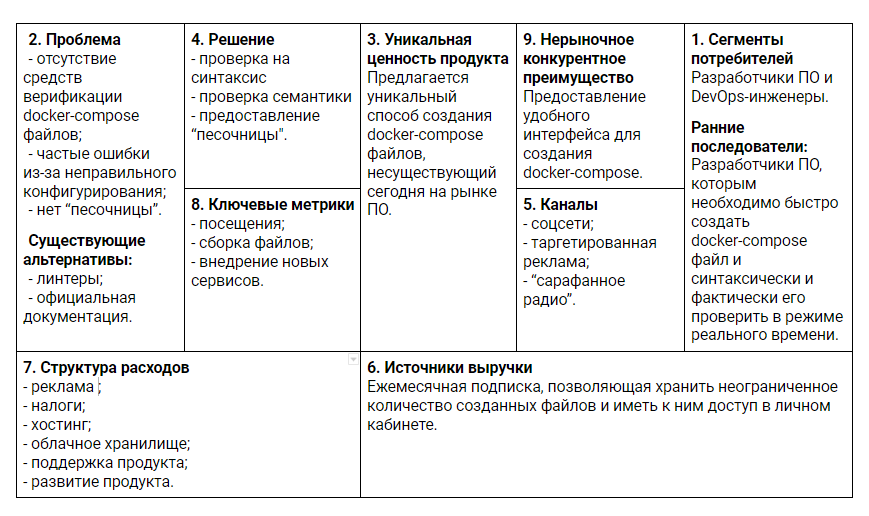
\includegraphics[scale=0.7]{canvas.png}}
    \caption{Экономическое описание стартапа}
    \label{ec:canvas}
\end{figure}

\tocless\subsection{Расчёт прямых расходов}

Прямые расходы включают в себя:
\begin{itemize}
    \item Расходы на оплату труда с учётом трудозатрат;
    \item Страховые взносы во внебюджетные фонды
\end{itemize}

\subsubsection{Расчёт расходов на оплату труда}

Разработкой проекта будут заниматься backend-разработчик и
frontend-разработчик.

Их заработная плата составляет по 30 000 руб. в месяц.

\begin{equation}
   \text{ФОТ}_\text{год} = \text{ЗП} * 12 \text{мес},
\end{equation}

\begin{eqexpl}[5ex]
    \item{ФОТ} Фонд оплаты труда, руб.;
    \item{ЗП} Заработная плата, руб.;
\end{eqexpl}

\begin{equation*}
    \text{ФОТ}_\text{год} = 30 000 * 12 \text{мес.} = 30 000 \text{руб.}
\end{equation*}

Теперь определм стоимость трудозатрат в час по формуле \ref{ec:trudzat}:

\begin{equation}
    \label{ec:trudzat}
    \text{Ct}_\text{час} = \text{ФОТ} / N_\text{рв},
\end{equation}

\begin{eqexpl}[5ex]
    \item{$\text{Ct}_\text{час}$} Стоимость трудозатрат за 1 час, руб
    \item{$\text{N}_\text{рв},$} Норма рабочего времени при 40-ка часовой рабочей
неделе.
\end{eqexpl}

\begin{equation*}
    \text{Ct}_\text{час} = 360 000 / 1979 = 181,91 \text{руб}.
\end{equation*}

Теперь рассчитаем сумму расходов на оплату труда и каждый пункт
разработки занесём в таблицу \ref{ec:table1}.

\tabcolsep=0.1cm
\begin{longtable}[c]{|l|c|c|r|}
    \caption{Расчет расходов на оплату труда с учетом трудозатрат}
    \label{ec:table1}\\
    \hline
    \multicolumn{1}{|c|}{{\begin{tabular}[c]{@{}c@{}}Наименование\\ работ/услуг\end{tabular}}} &
      {\begin{tabular}[c]{@{}c@{}}Трудозатраты, \\ час\end{tabular}} &
      {\begin{tabular}[c]{@{}c@{}}Стоимость \\ трудозатрат в час, \\ руб\end{tabular}} &
      {\begin{tabular}[c]{@{}c@{}}Общая стоимость\\ работ, \\ руб\end{tabular}} \\ \hline
    \endfirsthead
    %
    \multicolumn{4}{l}%
    {{\hspace{5ex} Продолжение таблицы \thetable \vspace{0.5cm}}} \\ \hline
    \multicolumn{1}{|c|}{{\begin{tabular}[c]{@{}c@{}}Наименование\\ работ/услуг\end{tabular}}} &
    {\begin{tabular}[c]{@{}c@{}}Трудозатраты, \\ час\end{tabular}} &
    {\begin{tabular}[c]{@{}c@{}}Стоимость \\ трудозатрат в час, \\ руб\end{tabular}} &
    {\begin{tabular}[c]{@{}c@{}}Общая стоимость\\ работ, \\ руб\end{tabular}} \\ \hline    \endhead
    %
    \begin{tabular}[c]{@{}l@{}}Разработка\\ требований\end{tabular}                              & 72            & 181,91          & 13097,52           \\ \hline
    \begin{tabular}[c]{@{}l@{}}Создание прототипов\\ пользовательского\\ интерфейса\end{tabular} & 16            & 181,91          & 2910,56            \\ \hline
    \begin{tabular}[c]{@{}l@{}}Написание прототипа\\ сервера\end{tabular}                        & 36            & 181,91          & 6548,76            \\ \hline
    Создание дизайна                                                                             & 32            & 181,91          & 5821,12            \\
    \pagebreak
    \begin{tabular}[c]{@{}l@{}}Разработка общей\\ архитектуры проекта\end{tabular}               & 56            & 181,91          & 10186,91           \\ \hline
    Выбор технологий                                                                             & 24            & 181,91          & 4365,84            \\ \hline
    \begin{tabular}[c]{@{}l@{}}Написание кода\\ клиентской части\end{tabular}                    & 496           & 181,91          & 90227,36           \\ \hline
    \begin{tabular}[c]{@{}l@{}}Написание кода\\ серверной части\end{tabular}                     & 456           & 181,91          & 82950,96           \\ \hline
    \begin{tabular}[c]{@{}l@{}}Тестирование клиентской\\ части\end{tabular}                      & 40            & 181,91          & 7276,41            \\ \hline
    \begin{tabular}[c]{@{}l@{}}Тестирование сервеной\\ части\end{tabular}                        & 24            & 181,91          & 4365,84            \\ \hline
    Написание документации                                                                       & 8             & 181,91          & 1455,28            \\ \hline
    \begin{tabular}[c]{@{}l@{}}Изучение документаций к\\ выбранным технологиям\end{tabular}      & 24            & 181,91          & 4365,84            \\ \hline
    Развёртывание на сервере                                                                     & 24            & 181,91          & 4365,84            \\ \hline
    {Итого}                                                                                      & 1308          & 181.91          & 237938,28          \\ \hline
\end{longtable}

\subsubsection{Расчёт страховых взносов во внебюджетные фонды}

Следующим шагом будет определение страховых взносов во внебюджетные фонды, которые состоят
из следующих тарифов:

\begin{itemize}
    \item на обязательное пенсионное страхование ~--- 22,0\%;
    \item на обязательное социальное страхование на случай временной нетрудоспособности и в связи с материнством ~--- 2,9\%;
    \item на обязательное медицинское страхование ~--- 5,1\%;
    \item на обязательное социальное страхование от несчастных случаев на производстве и профессиональных заболеваний ~--- 0.2\%.
\end{itemize}

Для расчёта общих страховых взносов используется формула \ref{ec:strah}:

\begin{equation}
    \label{ec:strah}
    \text{C}_\text{страх-вз} = \text{ФОТ}_\text{год} * 30,2\% / 100\%,
\end{equation}

\begin{eqexpl}[7ex]
    \item{$\text{ФОТ}_\text{год}$} Фонд оплаты труда, руб.
\end{eqexpl}

\begin{equation*}
    \text{C}_\text{страх-вз} = 237938,28 * 30,2\% / 100\% = 71857,36 руб.
\end{equation*}

\tocless\subsection{Определение накладных расходов на разработку программного продукта}

Накладные расходы включают в себя следующие пункты:

\begin{itemize}
    \item Услуги связи(интернет, телефон);
    \item Коммунальные расходы;
    \item Расходы на рекламу;
    \item Прочие
\end{itemize}

Для расчёта накладных расходов рассчитаем временные сроки выполнения проекта по следующей
формуле:

\begin{equation}
    \text{СП} = t_\text{Общ} / 8,
\end{equation}

\begin{eqexpl}[5ex]
    \item{СП} Временные сроки выполнения, дн.;
    \item{$t_\text{общ}$} Общая сумма трудозатрат, час;
    \item{8} Стандартный рабочий день, час.
\end{eqexpl}

\begin{equation*}
    \text{СП} = 1308 / 8 = 163,5 дн.
\end{equation*}

\subsubsection{Расчёт расходов на услугуи связи}

Расчёт расходов на связь можно посчитать по следующей формуле:

\begin{equation}
    \text{P}_\text{y.c.} = (\text{P}_\text{интернет} + \text{P}_\text{тел.связь}) / \text{Кол-во дней(мес)} * \text{СП},
\end{equation}

\begin{eqexpl}[18ex]
    \item{$\text{P}_\text{интернет} + P_\text{тел.связь}$} Расходы на интернет, мобильную связь и т.д.;
    \item{Кол-во дней(мес)} Среднее количество рабочий дней в месяце, дн.
\end{eqexpl}

\begin{equation*}
    \text{P}_\text{y.c.} = (450 + 300 + 400 + 300) / 21 * 163,5 = 11289,29 руб.
\end{equation*}

\subsubsection{Расчёт расходов на коммунальные услуги}

Расчёт коммунальных услуг произведём по формуле \ref{ec:eq_com}:

\begin{equation}
    \label{ec:eq_com}
    \text{P}_\text{коммунальные} = \text{n}_\text{к.у} * \text{S} / \text{Кол-во дней(мес)} * \text{СП},
\end{equation}

\begin{eqexpl}[12ex]
    \item{$\text{P}_\text{коммунальные}$} Расходны на коммунальные услуги;
    \item{$\text{n}_\text{к.у}$} Средняя ставка на ком. услуги за 1 кв. метр;
    \item{$\text{S}$} Площадь помещения в кв. м.
\end{eqexpl}

\begin{equation*}
    \text{P}_\text{коммунальные} = 120 * 30 / 21 * 163,5 = 28028,57 \text{руб}.
\end{equation*}

\subsubsection{Расчёт расходов на рекламу}

Произведём расчёт расходов на рекламу по следующей формуле:

\begin{equation}
    \text{P}_\text{реклама} = POT * n_\text{реклама} / 100\%,
\end{equation}

\begin{eqexpl}[7ex]
    \item{$\text{P}_\text{реклама}$} Сумма расходов на рекламу, руб.;
    \item{$\text{POT}$} Расходы на оплату труда, руб.;
    \item{$n_\text{реклама}$} Норматив расходов на рекламу, руб.
\end{eqexpl}

\begin{equation*}
    \text{P}_\text{реклама} = 237938,28 * 10\% / 100\% = 23793,83 \text{руб}.
\end{equation*}

\subsubsection{Расчёт прочих расходов}

Рассчитаем расходы на оплату труда, которые являются процентом от расходов
на оплату труда как и расходы на рекламу, по формуле:

\begin{equation}
    \text{P}_\text{прочие} = \text{POT} * n_\text{прочие} / 100\%,
\end{equation}

\begin{eqexpl}[6ex]
    \item{$\text{P}_\text{прочие}$} Сумма прочих расходов, руб.;
    \item{$\text{n}_\text{прочие}$} Норматив прочих расходов, \%
\end{eqexpl}

\begin{equation*}
    \text{P}_\text{прочие} =  237938,28 * 10\% / 100\% = 23793,83 \text{руб}.
\end{equation*}

\subsubsection{Расчёт общей суммы накладных расходов}

Теперь можно определить общую сумма накладных расходов по формуле \ref{ec:nak}:

\begin{equation}
    \label{ec:nak}
    \text{P}_\text{Накладные} = \text{P}_\text{y.c.} + \text{P}_\text{коммунальные} + \text{P}_\text{реклама} + \text{P}_\text{прочие}.
\end{equation}

\begin{eqexpl}[9ex]
    \item{$\text{P}_\text{Накладные}$} Сумма накладных расходов, руб.
\end{eqexpl}

\begin{equation*}
    P_\text{Накладные} = 11289,29 + 3600 + 23793,83 * 2 = 86905,52 \text{руб.}
\end{equation*}

\tocless\subsection{Расчёт себестоимости работ по разработке программного продукта}

Себестоимость работ по проекту включает в себя:

\begin{itemize}
    \item Расходы на оплату труда;
    \item Страховые взносы;
    \item Накладые расходы.
\end{itemize}

Расчёт себестоимости работ по проекту, иными словами цену непосредственного создания
программного продукта, привидена в таблице \ref{ec:table2}.

\begin{longtable}[c]{|p{10cm}|r|}
    \caption{Себестоимость работ по созданию программного продукта}
    \label{ec:table2}\\
    \hline
    \multicolumn{1}{|c|}{{Статьи расходов}} & {\begin{tabular}[c]{@{}c@{}}Сумма, руб.\end{tabular}} \\ \hline
    \endfirsthead
    %
    \multicolumn{2}{c}%
    {{Продолжение таблицы \thetable}} \\
    \endhead
    %
    Расход на оплату труда & 237938,28          \\ \hline
    Страховые взносы       & 71857,36           \\ \hline
    Накладные расходы      & 86905,52           \\ \hline
    {Итого}         & 396701,16 \\ \hline
\end{longtable}

\tocless\subsection{Расчёт сумму выручки от реализации программного продукта}

Цена создания и реализации программного продукта ~--- она же выручка от
реализации проекта определяется по следующей формуле:

\begin{equation}
    \text{B}_\text{реал} = \text{C}_\text{p} + \text{П},
\end{equation}

\begin{eqexpl}[3ex]
    \item{$C_p$} Себестоимость работ, руб.;
    \item{П} Планируемый размер прибыли, руб.
\end{eqexpl}

Планируемый размер прибыли определяется по следующей формуле:

\begin{equation}
    \text{П} = \frac{C_p * H_r}{100\%},
\end{equation}

\begin{eqexpl}[5ex]
    \item{$\text{H}_\text{R}$} Уровень рентабельности проекта, \%.
\end{eqexpl}

Возьмём за уровень рентабельности 10\%, так как проект не прибыльный по своей сути.

\begin{equation*}
    \text{П} = \frac{396701,16 * 10\%}{100\%} = 39670,12 \text{руб}.
\end{equation*}

Следовательно:

\begin{equation*}
    \text{B}_\text{реал} = 396701,16 + 39670,12 = 436371,28 \text{руб.},
\end{equation*}

Основные же показатели, учитываемые при расчётё цены программного продукта привидены в таблице
\ref{ec:table3}

\begin{longtable}[c]{|l|r|}
    \caption{Расчет цены программного продукта}
    \label{ec:table3}\\
    \hline
    \multicolumn{1}{|c|}{{Наименование показателя}} & {Сумма, руб} \\ \hline
    \endfirsthead
    %
    \multicolumn{2}{c}%
    {{Продолжение таблицы \thetable}} \\
    \endhead
    %
    Затраты на создание программного продукта              & 396701,16           \\ \hline
    Прибыль                                                & 39670,12           \\ \hline
    Выручка от реализации проекта                          & 436371,28           \\ \hline
\end{longtable}

\tocless\subsection{Расчёт суммы единого налога при применении упрощённой системы налогообложения}

Произведём расчёт суммы единого налога по формуле:

\begin{equation}
    \text{УСН}_\text{нач} = \frac{\text{Д} * \text{C}_\text{усн}}{100\%},
\end{equation}

\begin{eqexpl}[7ex]
    \item{$\text{УСН}_\text{нач}$} Сумма единого налогового начисления, руб.;
    \item{Д} Доход, руб.;
    \item{$\text{C}_\text{усн}$} Ставка налога, \%.
\end{eqexpl}

\begin{equation*}
    \text{УСН}_\text{нач} = \frac{37227,259 * 6\%}{100\%} = 26182,28 \text{руб}.
\end{equation*}

Налогоплательщики, выбравшие в качестве объекта налогообложения
доходы, уменьшают сумму налога, исчисленную за налоговый период, на
сумму страховых взносов, но не более, чем на 50\%.

Определим сумму минимального налога по формуле:

\begin{equation}
    \text{УСН}_\text{min} = \frac{\text{УСН}_\text{нач} * 50\%}{100\%},
\end{equation}

\begin{eqexpl}[7ex]
    \item{$\text{УСН}_\text{min}$} Минимальная сумма налога, руб.
\end{eqexpl}

\begin{equation*}
    \text{УСН}_\text{min} = \frac{26182,28 * 50\%}{100\%} = 13091,14 руб.
\end{equation*}

Произведем расчет суммы единого налога, подлежащей перечислению
в бюджет по формуле:

\begin{equation}
    \text{УСН}_\text{бюджет} = \text{УСН}_\text{нач} - \text{УСН}_min
\end{equation}

\begin{equation}
    \text{УСН}_\text{бюджет} = 26182,28 - 13091,14 = 13091,14 руб.
\end{equation}

\tocless\subsection{Расчёт чистой прибыли организации}

Рассчитаем сумму чистой прибыли, остающаяся в распоряжении организации,
после уплаты единого налога по формуле:

\begin{equation}
    \text{П}_\text{чистая} = \text{П} - \text{УСН}_\text{бюджет},
\end{equation}

\begin{eqexpl}[7ex]
    \item{$\text{П}_\text{чистая}$} Планируемая сумма прибыли от реализации проекта, руб.
\end{eqexpl}

\begin{equation*}
    \text{П}_\text{чистая} = 39670,12 - 13091,14 = 26578,98 руб
\end{equation*}

Расчет чистой прибыли организации от разработки программного
продукта сведём в таблицу \ref{ec:table4}

\begin{longtable}[c]{|l|r|}
    \caption{Расчёт чистой прибыли организации от разработки
    программного продукта.}
    \label{ec:table4}\\
    \hline
    \multicolumn{1}{|c|}{{Наименование статей}} & {Сумма, руб} \\ \hline
    \endfirsthead
    %
    \multicolumn{2}{l}%
    {{Продолжение таблицы \thetable \vspace{0.5cm}}} \\ \hline
    \multicolumn{1}{|c|}{{Наименование статей}} & {Сумма, руб} \\ \hline
    \endhead
    %
    Себестоимость работ по проекту                     & 396701,16          \\ \hline
    Планируемая сумма прибыли                          & 39670,12           \\
    \pagebreak
    Выручка от реализации проекта                      & 436371,28          \\ \hline
    Сумма единого налога, подлежащая уплате в бюджет   & 13091,14            \\ \hline
    \begin{tabular}[c]{@{}l@{}}Прибыль, остающаяся в распоряжении организации,\\ после уплаты единого налога при применении УСН\end{tabular} & 26578,98 \\ \hline
\end{longtable}

\tocless\subsection{Расчёт стоимости владения программным продуктом}

Стоимость владени программным продуктом включает в себя
эксплуатационные расходы (Эр) на обслуживание разработанного
программного продукта (таблица \ref{ec:table5}), измеряются в часах, затраченных на
указанные ниже виды работ.

Ежемесячные затраты на функционирование (Зф) программного
продукта (таблица \ref{ec:table6}) так же входят в стоимость владения программным
продуктом.

\tabcolsep=0.1cm
\begin{longtable}[c]{|l|c|c|r|}
    \caption{Расчет эксплуатационных расходов.
    }
    \label{ec:table5}\\
    \hline
    \multicolumn{1}{|c|}{{Наименование статей}} &
      \begin{tabular}[c]{@{}c@{}}Количество\\ часов,\\ час/мес\end{tabular} &
      \begin{tabular}[c]{@{}c@{}}Стоимость\\ трудозатрат в\\ час, \\ руб.\end{tabular} &
      \begin{tabular}[c]{@{}c@{}}Сумма,\\ руб. в месяц\end{tabular} \\ \hline
    \endfirsthead
    %
    \multicolumn{4}{c}%
    {{Продолжение таблицы \thetable}} \\
    \endhead
    %
    Создание новых сервисов                                                                                         & 24          & 181.91          & 4365,84           \\ \hline
    Оптимизация производительсности                                                                                 & 10          & 181.91          & 1819,12            \\ \hline
    \begin{tabular}[c]{@{}l@{}}Установка и тестирование\\ программных обновлений\\ разработотанного ПО\end{tabular} & 5           & 181.91          & 909,55            \\ \hline
    Модерация ресурсов                                                                                              & 30          & 181.91          & 5457,32            \\ \hline
    Итого                                                                                                  & 69 & 181.91 & 12551,79 \\ \hline
\end{longtable}

\begin{longtable}[c]{|p{10cm}|r|}
    \caption{Расчет затрат на функционирование.
    }
    \label{ec:table6}\\
    \hline
    \multicolumn{1}{|c|}{{Виды затрат}}                                              & \begin{tabular}[c]{@{}c@{}}Сумма,\\ руб./месяц\end{tabular} \\ \hline
    \endfirsthead
    %
    \multicolumn{2}{c}%
    {{Продолжение таблицы \thetable}} \\
    \endhead
    %
    Стоимость домена   & 590           \\ \hline
    Стоимость хостинга & 825           \\ \hline
    \begin{tabular}[c]{@{}l@{}}Стоимость облачного\\ сервиса базы данных(mLab)\end{tabular} & 545                                                                  \\ \hline
    {Итого}     & {1960} \\ \hline
\end{longtable}

Итого, стоимость владения (Св) рассчитывается как сумма
эксплуатационных расходов и затрат на функционирование по формуле:

\begin{equation}
    \text{C}_\text{в} = \text{Э}_\text{р} + \text{З}_\text{ф}.
\end{equation}

\begin{equation*}
    \text{C}_\text{в} = 12551,79 + 1960 = 14511,79 руб.
\end{equation*}

Вывод: стоимость владения разработанным продуктом, составляет 14511,79 руб. в месяц.

\vspace{1.2cm}

\subsection{Смета затрат на проект}

Смета затрат на проект включает в себя себестоимость проекта,
заложенную сумму прибыли разработчика, сумму налоговых платежей.
Отдельной строкой необходимо указать стоимость владения программным
продуктом. Расчёт сметы представлен в таблице \ref{ec:table7}

\begin{longtable}[c]{|p{1.5cm}|p{11.5cm}|r|}
    \caption{Смета затрат на проект.}
    \label{ec:table7}\\
    \hline
    \multicolumn{1}{|c|}{{\begin{tabular}[c]{@{}c@{}}№\\ п/п\end{tabular}}} &
      \multicolumn{1}{c|}{{Статьи смета затрат на проект}} &
      {\begin{tabular}[c]{c@{}c@{}}Сумма, руб.\end{tabular}} \\ \hline
    \endfirsthead
    %
    \multicolumn{3}{l}{Продолжение таблицы \thetable \vspace{0.5cm}} \\ \hline
    \multicolumn{1}{|c|}{{\begin{tabular}[c]{@{}c@{}}№\\ п/п\end{tabular}}} &
    \multicolumn{1}{c|}{{Статьи смета затрат на проект}} &
    {\begin{tabular}[c]{@{}c@{}}Сумма, руб.\end{tabular}} \\ \hline
    \endhead
    %
    1 &
      \begin{tabular}[c]{@{}l@{}}Затратны на создание программного продукта\\ (себестоимость работ)\end{tabular} &
      396701,16 \\ \hline
                         & Расходы на оплату труда               & 237938,28  \\ \hline
                         & Страховые взносы                      & 71857,36   \\ \hline
                         & Накладные расходы                     & 86905,52   \\
    \pagebreak
    2                    & Чистая прибыль                        & 26578,98  \\ \hline
    3                    & Налог по УСН с выручки                & 13091,14   \\ \hline
    \multicolumn{2}{|l|}{Итого общая стоимость работ по проекту} & 436371,28 \\ \hline
    4                    & Стомость владения ПП, месяц           & 14511,79   \\ \hline
\end{longtable}

    \newpage
    \section{Техника безопасности и охрана труда}

\vspace{-0.9cm}

\tocless\subsection{Требования охраны труда перед началом работы}


Проверить:
    \begin{enumerate}
        \item корректность естественного освещения;
        \item исправность и корректность электроосвещения в кабинете (не менее 300-500 лк на поверхности стола в зоне размещения документа);
        \item площадь рабочего места (не менее 6 м2);
        \item объём рабочего места (не менее 20 м3);
        \item корректность расстояния между мониторами (между основными поверхностями мониторов – не менее 2 м, между боковыми их поверхностями – не менее 1,2 м);
        \item исправность и корректность рабочего кресла (должно быть с подлокотниками, подъёмно-поворотным, с устройством регулировки хода по высоте в пределах 400-550 мм и углам наклона вперёд-назад в пределах 5-15°).
    \end{enumerate}
Проверить работоспособность ПЭВМ, иных электроприборов, а также средств связи, находящихся в кабинете.

Проветрить помещение кабинета.

Проверить безопасность рабочего места на предмет стабильного положения и исправности мебели, измерительных приборов, инструментов, приспособлений, а также проверить наличие в достаточном количестве расходных материалов.

Уточнить план работы на день и, по возможности, распределить намеченное к исполнению равномерно по времени, с включением 15 мин. отдыха (либо кратковременной смены вида деятельности) через каждые 45 мин. однотипных производственных действий, а также с отведением времени в объёме не менее 30 мин. для приёма пищиориентировочно через 4-4,5 ч. луха, памяти, внимания - вследствие ром для решения тех или иных вопросов производственного хара.


\tocless\subsection{Требования охраны труда во время работы}


    Соблюдать правила личной гигиены.

    Исключить пользование неисправным электроосвещением, неработоспособными ПЭВМ, иными электроприборами, а также средствами связи, находящимися в кабинете.

    Поддерживать чистоту и порядок на рабочем месте, не загромождать его бумагами, книгами и т.п.

    Соблюдать правила пожарной безопасности.

    При 8-часовом рабочем дне следует соблюдать регламентированные (технологические) перерывы:
\begin{enumerate}
        \item при работе по считыванию информации с экрана ПЭВМ с предварительным запросом и суммарным числом считываемых знаков до 60 000 знаков за смену – 20 мин перерыва через 1,5-2 часа после начала рабочего дня и через 1,5-2 часа после обеденного перерыва; альтернативно – 15 мин через каждый час.
        \item при работе по считыванию информации с экрана ПЭВМ с предварительным запросом и суммарным числом считываемых знаков до 40 000 знаков за смену –  15 мин перерыва через 2 часа после начала рабочего дня и через 1,5-2 часа после обеденного перерыва; альтернативно – 10 мин через каждый час.
        \item при работе творческого характера в режиме диалога с ПЭВМ и продолжительностью работы до 6 ч за смену –  15 мин перерыва через 2 часа после начала рабочего дня и через 2 часа после обеденного перерыва.
\end{enumerate}


\tocless\subsection{Требования охраны труда в аварийных ситуациях}


    Не приступать к работе при плохом самочувствии или болезни.

    В случае возникновения аварийных ситуаций сообщить о случившемся инженеру по охране труда и технике безопасности или, в его отсутствие, дежурному администратору и далее действовать в соответствии с полученными указаниями, а также:

    В случае возникновения пожара руководствоваться соответствующим Планом эвакуации, инструкцией по противопожарной безопасности.

    В случае угрозы или в случае возникновения очага опасного воздействия техногенного характера руководствоваться соответствующим Планом эвакуации, инструкцией по организации мер безопасности в случае угрозы или в случае возникновения очага опасного воздействия техногенного характера.

    В случае угрозы или в случае приведения в исполнение террористического акта руководствоваться соответствующим Планом эвакуации, инструкцией по организации мер безопасности в случае угрозы или в случае приведения в исполнение террористического акта.

    При необходимости следует обратиться за помощью и (или) оказать первую помощь пострадавшим от травматизма.

    Оказать всемерное содействие расследованию несчастного случая.

\vspace{1.2cm}

\tocless\subsection{Требования охраны труда по окончанию работ}

Проветрить кабинет, закрыть окна.

Привести в порядок рабочее место.

Выключить электроприборы, ПЭВМ.

Выключить электроосвещение.

Настоящая Инструкция составлена с соблюдением требований действующего законодательства и производственных нормативов, утверждённых постановлением Министерства труда и социального развития РФ от 17.12.2002 №80.
    \newpage
    \section{Сведения о внедрении}

Проект размещён на хостинге и доступен по адресу configcastle.ru

Обо серверых приложений размещёны на сервисе heroku и отслает результат клиенту, распложенному на хостинге firebase.

    \newpage
    \section*{\centersection{Заключение}}

В ходе выполнения выпускной квалификационной работы был проведён сбор требований и их дальнейший анализ
для наиболее правильного проектирования, произошедшего в дальнейшем.
В процессе дизайна продукта были созданы прототипы, выбрана база данных и создана
общая архитектура приложения. Инструменты также были подобраны под условия разработки и
и обоснованы.

Продукт в дальнейшем может развиваться, привнося новые виды конфигурационных файлов, тем самым привлекая новых пользователей.

Проект выполнен с учётом последних технологий, используя новые подходы и билиотеки, такие как бекенд, обрабатывающий запросы асинхронно и GraphQL.
Тестирование проекта также было выполнено, выявив некоторые ошибки в ходе выполнения приложения. Весь код проекта был выложен
на github как свободное программное обеспечение и доступен по ссылке: https://github.com/configCastle.
    \newpage
    \section*{\centersection{Список литературы}}
\addcontentsline{toc}{section}{Список литературы}

\begin{enumerate}[label=\arabic*]
    \item Пузыревский И.А. Правила оформления текстовых документов в учебном процессе. ­– 8-е изд. – Ростов-на-Дону: РКСИ, 2012 г.
    \item Критерии оценки качества подготовки ВКР по рейтинговой системе для специальности 09.02.03 «Программирование в компьютерных системах». – Ростов-на-Дону: РКСИ, 2020 г.
    \item Порселло Ева, Бэнкс Алекс. GraphQL. Язык запросов для современных веб-приложений - изд. Прогресс книга, 2019 г.
    \item Лутц Марк. Изучаем Python. Том 1 - изд. Вильямс, 2019 г.
    \item Лутц Марк. Изучаем Python. Том 2 - изд. Вильямс, 2019 г.
    \item Лутц Марк. Python. Кармананный справочник. - изд. Вильямс, 2016 г.
    \item Caleb Hattingh. Using Asyncio in Python: Understanding Python's Asynchronous Programming Features - изд. O'Reilly, 2020 г.
    \item Эдриен Моуэт. Использование Docker. Разработка и внедрение программного обеспечения при помощи технологии контейнеров - изд. ДМК, 2017 г.
    \item Эрик Редмонд. Джим. Р. Уилсон. Семь баз данных за семь недель. Введение в современные базы данных и идеологию NoSQL. - изд. ДМК, 2013 г.
    \item Documentation generator and online help system[Электронный ресурс] - Режим доступа: https://docs.python.org/3.8/library/pydoc.html - Загл. с экрана.
    \item Getting started with Tartiflette[Электронный ресурс] - Режим доступа: https://tartiflette.io/docs/tutorial/getting-started - Загл. с экрана.
    \item Что такое Docker?[Электронный ресурс] - Режим доступа: https://aws.amazon.com/ru/docker/ - Загл. с экрана.
    \item Overview of Docker Compose[Электронный ресурс] - Режим доступа: https://docs.docker.com/compose/ - Загл. с экрана.
    \item Test Plan Template(IEEE 829-1998 Format)[Электронный ресурс] - Режим доступа: http://www.ecs.csun.edu/\~{}rlingard/comp480/TestPlanTemplate.pdf - Загл. с экрана
    \item PEP 8 -- Style Guide for Python Code[Электронный ресурс] - Режим доступа: https://www.python.org/dev/peps/pep-0008/ - Загл. с экрана.
    \item Tutorial: Using Motor With asyncio[Электронный ресурс] - Режим доступа: https://motor.readthedocs.io/en/stable/tutorial-asyncio.html - Загл. с экрана.
\end{enumerate}

    \newpage
    \section*{\hfill ПРИЛОЖЕНИЕ А \\ \hspace*{13.5cm} (обязательное)}
\addcontentsline{toc}{section}{Приложение А}


1 Фрагмет кода модуля mutation\_resolvers:

\begin{Verbatim}
        """Module for mutation."""
        from bson.objectid import ObjectId
        from tartiflette import Resolver

        from algernon.utils.db import 

        @Resolver('Mutation.createFile')
            async def resolve_mutation_create_file(parent, args, ctx, system):
            """
            Resolve mutation createFile in GraphqQL API.
            Args:
                parent: initial field in 'execute' method
                args: argument for query
                ctx: context field
                system: information related to the execution
            Returns:
                return created document
            """
            db = ctx['req'].app['db']

            file_id = await return_last_id(db, 'file') + 1

            document = await db['file'].insert_one(
                {
                    'id': file_id,
                    'name': args['input']['name'],
                    'data': args['input']['data'],
                    'configType': args['input']['configType'],
                },
            )

            return await db['file'].find_one(
                {'_id': ObjectId(document.inserted_id)}
            )

        @Resolver('Mutation.deleteFile')
        async def resolve_mutation_delete_file(parent, args, ctx, system):
            """
            Resolve mutation deleteFile in GraphqQL API.
            Args:
                parent: initial field in 'execute' method
                args: argument for query
                ctx: context field
                system: information related to the execution
            Raises:
                Exception: If 'id' of document not found
            Returns:
                Removed document
            """
            db = ctx['req'].app['db']

            document = await db.file.find_one({'id': args['id']})

            if document is None:
                raise Exception('File does not exist.')

            db.file.delete_one({'id': args['id']})

            return document

        @Resolver('Mutation.updateFile')
        async def resolve_mutation_update_file(parent, args, ctx, system):
            """
            Resolve mutation updateFile in GraphqQL API.
            Args:
                parent: initial field in 'execute' method
                args: argument for query
                ctx: context field
                system: information related to the execution
            Raises:
                Exception: If 'id' of document not found
                Exception: If new data not input
            Returns:
                Updated document
            """
            db = ctx['req'].app['db']

            args_input = args['input']

            doc_base = {
                'name': None,
                'configType': None,
                'data': None,
            }

            doc_base['name'] = args_input.get('name')
            doc_base['configType'] = args_input.get('configType')
            doc_base['data'] = args_input.get('data')

            if all(file_value is None for file_value in doc_base.values()):
                raise Exception(
                    "You should provide at least one value: 'name'" +
                    "'type' or 'data'",
                )

            doc_base = {
                key: input_value for key, input_value in doc_base.items()
                if input_value is not None
            }

            if await db.file.find_one({'id': args_input['id']}) is None:
                raise Exception('File does not exist.')

            await db.file.update_one(
                {'id': args_input['id']},
                {'$set': doc_base},
            )

            return await db.file.find_one({'id': args_input['id']})
\end{Verbatim}

2. Фрагмет кода модуля query\_resolvers:

\begin{Verbatim}
        """Query resolovers for API."""
        from tartiflette import Resolver

        from algernon.utils.db import return_all


        @Resolver('Query.services')
        async def resolve_query_services(parent, args, ctx, system):
            """
            Resolve all services.
            Args:
                parent: initial field in 'execute' method
                args: argument for query
                ctx: context field
                system: information related to the execution
            Returns:
                all objects in collections
            """
            db = ctx['req'].app['db']

            return await return_all(db, 'service')


        @Resolver('Query.service')
        async def resolve_query_service(parent, args, ctx, system):
            """
            Resolve one service.
            Args:
                parent: initial field in 'execute' method
                args: argument for query
                ctx: context field
                system: information related to the execution
            Returns:
                one service
            """
            db = ctx['req'].app['db']

            for document in await return_all(db, 'service'):
                if document['id'] == args['id']:
                    return document
            return None


        @Resolver('Query.files')
        async def resolve_query_files(parent, args, ctx, system):
            """
            Resolve all files in system.
            Args:
                parent: initial field in 'execute' method
                args: argument for query
                ctx: context field
                system: information related to the execution
            Returns:
                all objects in collections
            """
            db = ctx['req'].app['db']

            return await return_all(db, 'file')


        @Resolver('Query.file')
            async def resolve_query_file(parent, args, ctx, system):
            """
            Resolve one file.
            Args:
                parent: initial field in 'execute' method
                args: argument for query
                ctx: context field
                system: information related to the execution
            Returns:
                one file
            """
            db = ctx['req'].app['db']

            for document in await return_all(db, 'file'):
                if document['id'] == args.get('id', None):
                    return document

            return None
\end{Verbatim}

    \newpage
\end{document}
